\documentclass[pldi,nocopyrightspace]{sigplanconf-pldi15}

\usepackage{amssymb,amsmath,amsthm}
\usepackage{latexsym}
\usepackage{graphicx}
\usepackage[usenames,dvipsnames]{color}
\usepackage{listings}
\usepackage{float}
\usepackage[scaled]{helvet}
\usepackage[noend]{algorithmic}
\usepackage{mathrsfs}
\usepackage{mathpartir}
\usepackage{dsfont}
\usepackage{stmaryrd}
\usepackage{url}
\usepackage{textcomp} 
\usepackage[colorlinks=true,allcolors=blue,breaklinks,draft=false]{hyperref}
\usepackage{titlesec}
\usepackage{parskip}
\usepackage{alltt}
\usepackage{bbm}
\usepackage{alltt}
\usepackage{verbdef}
\usepackage{xspace}
\usepackage{verbatim}
\usepackage{enumitem}
\usepackage{lipsum}
\usepackage{doi}
%\usepackage[strut=on,font=footnotesize,labelfont=bf]{caption}
\usepackage[strut=on,labelfont=bf]{caption}

\usepackage{natbib}
\bibpunct();A{},
\let\cite=\citep

% For turned column headers 
\usepackage{adjustbox} 
\usepackage{array}
\usepackage{booktabs}
\usepackage{multirow}
\usepackage{pifont}
 
%%%%%%%%%%%%%%%%%%%%%%%%%%%%%%%%%%%%%%%%%%%%%%%%%%%%%%%%%%%%%%%%%%%%%%
% Compiling two paper versions
%%%%%%%%%%%%%%%%%%%%%%%%%%%%%%%%%%%%%%%%%%%%%%%%%%%%%%%%%%%%%%%%%%%%%%

\newcommand{\ifext}[2]{\ifdefined\extflag{#1}\else{#2}\fi}
\newcommand{\ifcomm}[1]{\ifdefined\extcomm{#1}\else{}\fi}

\newcommand{\mute}[1]{\ifdefined\draftflag{#1} \else{} \fi}
%\newcommand{\mute}[1]{}

\usepackage{skull}

\newcounter{ToDos}
\newcounter{WarnCounts}
\newcommand{\decorateWC}{
  \stepcounter{WarnCounts}
  \marginpar{\textcolor{red}{$\skull\ \theWarnCounts$}}}

\newcommand{\decorateTD}{
  \stepcounter{ToDos}
  \marginpar{\textcolor{red}{$\textbf{TO DO}_{\#\ \theToDos}$}}}


% Skeleton for remark comments
% 1: Name, 2: Color, 3:Comment
\newcommand{\signedComment}[3]
           {\mute{\textcolor{#2}{(#1: {#3})}\decorateWC}}

% remarks
\newcommand{\todo}[1]{\mute{\textcolor{red}{(TO DO:{#1})}\decorateTD}}

\newcommand{\is}[1]{\signedComment{Ilya}{blue}{#1}}
\newcommand{\an}[1]{\signedComment{Aleks}{red}{#1}}
\newcommand{\ab}[1]{\signedComment{AB}{red}{#1}}
\newcommand{\gad}[1]{\signedComment{GAD}{red}{#1}}

\newcommand{\highlight}[1]
           {\ifdefined\draftflag{{\textcolor{red}{#1}}} \else{#1} \fi}

\newenvironment{draft}
           {\ifdefined\draftflag \par\color{red} \else \comment \fi}
           {\ifdefined\draftflag \decorateWC\par \else \endcomment \fi}
           
% useful macros
\newcommand{\asgn}{\leftarrow}
\newcommand{\code}[1]{\lstinline[basicstyle=\small\ttfamily]{#1}}
\newcommand{\ccode}[1]{\lstinline[basicstyle=\footnotesize\ttfamily]{#1}}
\newcommand{\cccode}[1]{\lstinline[basicstyle=\scriptsize\ttfamily]{#1}} 
\newcommand{\Code}[1]{\code{#1}}
\newcommand{\etc}{\emph{etc}}
\newcommand{\ie}{\emph{i.e.}\xspace}
\newcommand{\id}{\emph{Id.}\xspace}
\newcommand{\eg}{\emph{e.g.}\xspace}
\newcommand{\vs}{\emph{vs.}\xspace}
\newcommand{\etal}{\emph{et~al.}\xspace}
\newcommand{\adhoc}{\emph{ad~hoc}\xspace}
\newcommand{\viz}{\emph{viz.}\xspace}
\newcommand{\dom}[1]{\mathsf{dom}(#1)}
\newcommand{\aka}{\textit{a.k.a.}\xspace}
\newcommand{\cf}{\textit{cf.}\xspace}
\newcommand{\wrt}{{wrt.}\xspace}
\newcommand{\Iff}{{iff}\xspace}
\newcommand{\loef}{L\"{o}f}
\newcommand{\sep}{\textasteriskcentered}
\newcommand{\res}{\mathsf{res}}
\newcommand{\bal}{\mathit{bal}} 
\newcommand{\ret}{\mathsf{ret}} 
\newcommand{\fix}{\mathsf{fix}} 
\newcommand{\Unit}{\mathsf{Unit}}  
\newcommand{\ic}{\mathcal{I}}
\newcommand{\Ic}[2]{\ic~{#1}~{#2}}
\newcommand{\hide}{\mathsf{hide}}  
\newcommand{\last}{\mathsf{last}}  

%specs
\newcommand{\specK}[1]{\ensuremath{\textcolor{blue}{#1}}}
\newcommand{\comm}[1]{\ensuremath{\textcolor{gray}{\esc{/\!/}~{#1}}}}
\newcommand{\spec}[1]{\specK{\left\{{#1}\right\}}}
\newcommand{\specQ}[4]{[#1 , #2 , #3] \, #4}%\specQ{mL}{gL}{gE}{p}
\newcommand{\drspec}[1]{\specK{\langle{#1}\rangle}}
\newcommand{\sspec}[1]{\specK{\{{#1}\}}}
\newcommand*{\backin}{\rotatebox[origin=c]{-180}{$\in$}}%

%actions
\newcommand{\act}[1]{\textsf{\small{#1}}}
\newcommand{\aux}[1]{\textit{#1}}
\newcommand{\Aux}[1]{\(\mathit{\small{#1}}\)}
\newcommand{\Num}[1]{{\text{{\scriptsize{#1}}}}}
\newcommand{\esc}[1]{\text{\texttt{\small{#1}}}}
\newcommand{\kw}[1]{\text{\textbf{#1}}}
\newcommand{\tp}[1]{\text{\textsf{#1}}}
\newcommand{\Asgn}{\leftarrow} 

%PCMs
\newcommand{\dotcup}{\ensuremath{\mathaccent\cdot\cup}}
\newcommand{\pcmS}{\mathbb{U}}
\newcommand{\pcmF}{\bullet}
\newcommand{\join}{\pcmF}
\newcommand{\jjoin}[1]{\ensuremath{\bigodot}_{#1=1}^n} 
\newcommand{\pcmU}{\mathbbm{1}}

% Pretty table
\newcommand{\cmark}{\ding{52}}%
\newcommand{\xmark}{\ding{55}}%
\newcommand*\rot{\rotatebox{32}} 
\newcommand{\yep}{\ding{51}}
\newcommand{\yepl}{$\text{\ding{51}}_{\!\!L}$}  
\newcommand{\yepa}{$\text{\ding{51}}_{\!\!L}$}  
\newcommand{\intab}[1]{({\sffamily{\small{#1}}})}

% Concurroids
\newcommand{\acon}{\mathcal{A}}
\newcommand{\econ}{\mathcal{E}}
\newcommand{\ucon}{\mathcal{U}}
\newcommand{\rcon}{\mathcal{R}}
\newcommand{\ccon}{\mathcal{C}}
\newcommand{\vcon}{\mathcal{V}}
\newcommand{\wcon}{\mathcal{W}}
\newcommand{\privcon}{\mathcal{P}}
\newcommand{\pscon}{\mathcal{S}}
\newcommand{\tbcon}{\mathcal{T}}
\newcommand{\fccon}{\mathcal{F}}
\newcommand{\lcon}{\mathcal{L}}
\newcommand{\alloccon}{\mathcal{A}}
\newcommand{\jayanticon}{\mathcal{J}}

%Getters
\newcommand{\lcl}{{\mathsf{s}}}%L
\newcommand{\env}{{\mathsf{o}}}%E
\newcommand{\joint}{{\mathsf{j}}}%E

\newcommand{\selfsub}{\mathsf{s}}
\newcommand{\othersub}{\mathsf{o}}
\newcommand{\jointsub}{\mathsf{j}}

\newcommand{\hist}{\chi} 
\newcommand{\histS}{\hist_{\, \selfsub}}
\newcommand{\histO}{\hist_{\, \othersub}}
\newcommand{\histJ}{\hist_{\, \jointsub}}
\newcommand{\hempty}{\emptyset}
\def\envsteps{\rightarrow^{*}_{\epsilon}}

\newcommand{\heap}{h} 
\newcommand{\heapS}{\heap_{\, \selfsub}}
\newcommand{\heapSP}{\heap_{\, \selfsub}'}

% Jayanti's Snapshot getters

\def\ordlist{\sigma}
\newcommand{\E}{\tau}
\newcommand{\C}{\kappa}


% Jayanti's Snapshot Orders
\newcommand{\tleq}{\mathrel{\leq_\ordlist}}
\newcommand{\tle}{\mathrel{<_\ordlist}}

\newcommand{\stableorder}{\Omega}
\newcommand{\prefix}[1]{-\,{\tleq}\,#1}

% Primed getters

\def\ordlistP{\sigma'}
\newcommand{\stableorderP}{\stableorder'}
\newcommand{\prefixP}[1]{(\mathrel{\tleqP}#1)}
\newcommand{\tleP}{\mathrel{<_\ordlistP}}
\newcommand{\tleqP}{\mathrel{\leq_\ordlistP}}
\newcommand{\EP}{\tau'}
\newcommand{\CP}{\kappa'}
\newcommand{\histP}{\chi'} 
\newcommand{\histSP}{\hist_{\, \selfsub}'}
\newcommand{\histOP}{\hist_{\, \othersub}'}
\newcommand{\histJP}{\hist_{\, \jointsub}'}

\newcommand{\wxP}{W_\x'}
\newcommand{\wyP}{W_\y'}
\newcommand{\wppP}{W_p'}

\newcommand{\jge}{\mathrel{>_\ordlist}}

\def\lgVy{\ensuremath{\mathsf{lastGY}}}


%% Writer and scanner states.

\newcommand{\wInit}{\mathsf{W_{Off}}}
\newcommand{\wWrite}{\mathsf{New}}
\newcommand{\wDirty}{\mathsf{Fwd}}
\newcommand{\wClean}{\mathsf{Done}}

\newcommand{\sOn}{\mathsf{S_{On}}}
\newcommand{\sOff}{\mathsf{S_{Off}}}

%mapsto stuff
\makeatletter
\newcommand{\oset}[3][0ex]{%
  \mathrel{\mathop{#3}\limits^{
    \vbox to#1{\kern-3\ex@
    \hbox{$\scriptstyle#2$}\vss}}}}
\makeatother

\makeatletter
\newcommand{\ojset}[3][0ex]{%
  \mathrel{\mathop{#3}\limits^{
    \vbox to#1{\kern-5\ex@
    \hbox{$\scriptstyle#2$}\vss}}}}
\makeatother

\newcommand{\jpts}{\mathrel{\ojset{j}{\mapsto}}}
\newcommand{\spts}{\mathrel{\oset{s}{\mapsto}}}
\newcommand{\opts}{\mathrel{\oset{o}{\mapsto}}}
\newcommand{\qcl}{\mathsf{cn}}

\newcommand{\hunion}{\mathbin{\dotcup}} 
\newcommand{\Hunion}[1]{\mathbin{\Dotcup{#1}}}

%% operators

\newcommand{\eqdef}{\mathrel{\:\widehat{=}\:}}
\newcommand{\hpts}{\mapsto}
\newcommand{\ldot}{\mathord{.}\,}

%% \newcommand{\aand}{,}
%% \newcommand{\oor}{\vee}
%% \newcommand{\nnot}{\neg}
%% \newcommand{\eqq}{\mathrel{\mbox{\tt==}}}
%% \newcommand{\neqq}{\mathrel{\mbox{\tt!=}}}
%% \newcommand{\andb}{\mathrel{\small\mbox{\&\&}}}
%% \newcommand{\orb}{\mathrel{\mbox{\tt{|\!|}}}}
%% \newcommand{\evar}[1]{?#1}
%% \newcommand{\zig}{\triangleleft}
%% \newcommand{\zag}{\triangleright}
%% \newcommand{\set}[1]{\left\{#1\right\}}
%% \newcommand{\tauflip}{\mathsf{flip\_trans}}
%% \newcommand{\tauadd}{\mathsf{add2\_trans}}
%% \newcommand{\tfr}[2]{{\text{fresh}^{#2}_{#1}}}

%% % more invariants
%% \newcommand{\tapprox}{\mathsf{ResInterf}}
%% \newcommand{\happrox}{\mathsf{ResPast}}
%% %\newcommand{\sapprox}{\mathsf{ResState}}
%% \newcommand{\bapprox}{\mathsf{ValuesMono}}
%% \newcommand{\strapprox}{\mathsf{IncResult}}
%% \newcommand{\Thisz}{\mathsf{this}}
%% \newcommand{\This}[1]{\Thisz~{#1}}

%% \newcommand{\hvalid}{\mathsf{Valid}}
%% \newcommand{\eqqc}{e_{\mathit{qqc}}}
%% \newcommand{\eqc}{e_{\mathit{qc}}}

%% \newcommand{\pending}{{m_\joint}} 
%% \newcommand{\offers}{h}
%% \newcommand{\twin}[1]{\bar{#1}}
%% \newcommand{\mygathjyer}[1]{|\!|{#1}|\!|}

%% \definecolor{shadecolor}{gray}{1.00}
%% \definecolor{ddarkgray}{gray}{0.75}
%% \definecolor{darkgray}{gray}{0.30}
%% \definecolor{light-gray}{gray}{0.87}
%% \newcommand{\whitebox}[1]{\colorbox{white}{#1}}
%% \newcommand{\graybox}[1]{\colorbox{light-gray}{#1}}
%% \newcommand{\darkgraybox}[1]{\colorbox{ddarkgray}{#1}}
%% \newcommand{\gbm}[1]{\graybox{${#1}$}}



%%% Snapshots paper related
%%%

\def\FF{\mathsf{False}}
\def\TT{\mathsf{True}}


%%% Specs
\newcommand{\tsPre}[1]{\ensuremath{{\textcolor{blue}{#1}}}}
\newcommand{\tsPos}[1]{\ensuremath{\textcolor{blue}{#1}}}
\newcommand{\logvar}[1]{\ensuremath{\textcolor{blue}{[#1].}}}

\newcommand{\var}[1]{\mathit{#1}} 
\newcommand{\num}[1]{{\text{{\scriptsize{#1}}}}}


\newcommand{\hfilter}{\mathrel{\downarrow}}

%% \newcommand{\cevX}[2]{\cev{#1}_{#2}}

%% \makeatletter
%% \DeclareRobustCommand{\cev}[1]{%
%%   \mathpalette\do@cev{#1}%
%% }

%% \newcommand{\do@cev}[2]{%
%%   \fix@cev{#1}{+}%
%%   \reflectbox{$\m@th#1\vec{\reflectbox{$\fix@cev{#1}{-}\m@th#1#2\fix@cev{#1}{+}$}}$}%
%%   \fix@cev{#1}{-}%
%% }
%% \newcommand{\fix@cev}[2]{%
%%   \ifx#1\displaystyle
%%     \mkern#23mu
%%   \else
%%     \ifx#1\textstyle
%%       \mkern#23mu
%%     \else
%%       \ifx#1\scriptstyle
%%         \mkern#22mu
%%       \else
%%         \mkern#22mu
%%       \fi
%%     \fi
%%   \fi
%% }


\def\GYR{{\mathbf{{g^{+}}{y^{?}}{r^{*}}}}}
\def\RZ{{\mathbf{{{(g | y)^{+}}}{r^{*}}}}}

%% \def\GYR{{\mathbf{{\color{OliveGreen}{G^{+}}}\bullet%
%%                    \color{YellowOrange}{Y^{?}}}\bullet%
%%                    \color{WildStrawberry}{R^{*}}}}



% code

\def\lat{\langle}
\def\rat{\rangle}
\def\tbnd{\Asgn}
\newcommand{\actwrite}[2]{{#1}\,{:=}\,{#2}}

%\def\altsubseteq{\mathbin{\subseteq}}


% Keep footnotes on one page
\interfootnotelinepenalty=10000 

\setlength{\parindent}{0.15in}
\setlength{\topsep}{0cm}
\setlength{\parskip}{0pt}
\titlespacing*{\section}{0pt}{*0.8}{*0.8} 
\titlespacing*{\subsection}{0pt}{*0.8}{*0.5}
\titlespacing*{\subsubsection}{0pt}{*0.8}{*0.5}
\titlespacing*{\paragraph}{0pt}{*0.3}{*0.3}

% SSReflect listings 
% colors
\definecolor{shadecolor}{gray}{1.00}
\definecolor{darkgray}{gray}{0.30}
\definecolor{violet}{rgb}{0.56, 0.0, 1.0}
\definecolor{forestgreen}{rgb}{0.13, 0.55, 0.13}

% Col language definition
\lstdefinelanguage{Coq} {
mathescape=true,						
texcl=false,
morekeywords=[1]{
  Add,
  All,
  Arguments,
  Axiom,
  Bind,
  Canonical,
  Check,
  Close,
  CoFixpoint,
  CoInductive,
  Coercion,
  Contextual,
  Corollary,
  Defined,
  Definition,
  Delimit,
  End,
  Example,
  Export,
  Fact,
  Fixpoint,
  Goal,
  Graph,
  Hint,
  Hypotheses,
  Hypothesis,
  Implicit,
  Implicits,
  Import,
  Inductive,
  Lemma,
  Let,
  Local,
  Locate,
  Ltac,
  Maximal
  Module,
  Morphism,
  Next,
  Notation,
  Obligation,
  Open,
  Parameter,
  Parameters,
  Prenex,
  Print,
  Printing,
  Program,
  Projections,
  Proof,
  Proposition,
  Qed,
  Record,
  Relation,
  Remark,
  Require,
  Reserved,
  Resolve,
  Rewrite,
  Save,
  Scope,
  Search,
  Section,
  Show,
  Strict,
  Structure,
  Tactic,
  Theorem,
  Unset,
  Variable,
  Variables,
  View,
  inside,
  outside
},
morekeywords=[2]{
  as,
  cofix,
  else,
  end,
  exists,
  exists2,
  fix,
  for,
  forall,
  fun,
  if,
  in,
  is,
  let,
  match,
  nosimpl,
  of,
  return,
  struct,
  then,
  vfun,
  with
},
morekeywords=[3]{Type, Prop, Set, True, False},
morekeywords=[4]{
  apply,
  assert,
  auto,
  bool_congr,
  case,
  change,
  clear,
  compute,
  congr,
  cut,
  cutrewrite,
  destruct,
  elim,
  field,
  fold,
  generalize,
  have,
  heval, 
  hnf,
  induction,
  injection,
  intro,
  intros,
  intuition,
  inversion,
  left,
  loss,
  move,
  nat_congr,
  nat_norm,
  pattern,
  pose,
  refine,
  rename,
  replace,
  revert,
  rewrite,
  right,
  ring,
  set,
  simpl,
  split,
  suff,
  suffices,
  symmetry,
  transitivity,
  trivial,
  unfold,
  using,
  without,
  wlog,
  autorewrite
},        
morekeywords=[5]{
  assumption,
  by,
  contradiction,
  done,
  exact,
  lia,
  gappa,
  omega,
  reflexivity,
  romega,
  solve,
  tauto,
  discriminate,
  unsat
},
morecomment=[s]{(*}{*)},
morekeywords=[6]{do, last, first, try, idtac, repeat},
showstringspaces=false,
morestring=[b]",
% Size of tabulations
tabsize=3,							
% Enables ASCII chars 128 to 255
extendedchars=true,  		 		
% Case sensitivity
sensitive=true, 
% Automatic breaking of long lines
breaklines=false,
% Default style fors listings
basicstyle=\small\ttfamily,
% Position of captions is bottom
captionpos=b,							
% Full flexible columns 
columns=[l]fullflexible,
% Style for (listings') identifiers
identifierstyle={\color{black}},
% Style for declaration keywords
keywordstyle=[1]{\color{violet}},
% Style for gallina keywords
keywordstyle=[2]{\color{forestgreen}},
% Style for sorts keywords
keywordstyle=[3]{\color{forestgreen}},
% Style for tactics keywords
keywordstyle=[4]{\color{blue}},
% Style for terminators keywords
keywordstyle=[5]{\color{red}},
%Style for iterators
keywordstyle=[6]{\color{violet}},
% Style for strings
stringstyle=,
% Style for comments
commentstyle=\it\ttfamily\color{Bittersweet},
% Style for lines numbering
numberstyle=\tiny,
}

\lstdefinestyle{Coq}{language=Coq}
\lstset{style=Coq}

% Hyphenation
\hyphenation{Veri-Fast}

% Bibtgex tweaks
\setcitestyle{square}
\defcitealias{Coq-manual}{Coq proof assistant}

\begin{document}

%\special{papersize=8.5in,11in}


% \authorinfo{Ilya Sergey}
%            {IMDEA Software Institute}
%            {ilya.sergey@imdea.org}
% %
% \authorinfo{Aleksandar Nanevski}
%            {IMDEA Software Institute}
%            {aleks.nanevski@imdea.org}

% \authorinfo{Anindya Banerjee}
%            {IMDEA Software Institute}
%            {anindya.banerjee@imdea.org}

\authorinfo{}


% \title{
% Mechanized Verification of Fine-grained Concurrent Programs 
% }

\title{
Mechanized Verification of Fine-grained Concurrent Programs 
\vspace{-65pt}
}
 

%\subtitle{}

\maketitle

\begin{abstract}

  Efficient concurrent programs and data structures rarely employ
  coarse-grained synchronization mechanisms (\ie,~locks); instead,
  they implement custom synchronization patterns via fine-grained
  primitives, such as \emph{compare-and-swap}.
  % 
  Due to sophisticated interference scenarios between threads,
  reasoning about such programs is challenging and error-prone, and
  can benefit from mechanization.
  
  In this paper, we present the first completely formalized framework for
  mechanized verification of \emph{full functional correctness} of
  fine-grained concurrent programs. Our tool is based on the recently
  proposed program logic FCSL.
  %
  It is implemented as an embedded domain-specific language in the
  dependently-typed language of the Coq proof assistant, and is
  powerful enough to reason about programming features such as
  higher-order functions and local thread spawning. By incorporating a
  uniform concurrency model, based on \emph{state-transition systems}
  and \emph{partial commutative monoids}, FCSL makes it possible to
  build proofs about concurrent libraries in a thread-local,
  compositional way, thus facilitating scalability and reuse:
  libraries are verified \emph{just once}, and their specifications
  are used ubiquitously in client-side reasoning.
  %
  We illustrate the proof layout in FCSL by example, and report on
  our experience of using FCSL to verify a number of concurrent
  algorithms and data structures.

\end{abstract}


\section{Introduction}
\label{sec:intro}

It has been long recognized that efficient parallelization is of
crucial importance for high-performant software. Unfortunately,
proving correctness of concurrent programs, in which several
computations can be executed in parallel, is difficult due to the
large number of possible interactions between concurrent
processes/threads on shared data structures.


% \ab{Can we also make the point that: fine-grained concurrent
%   algorithms are heavily used in concurrent data structure libraries
%   (cite?) and calls to such library functions in client code is
%   ubqiquitous (cite?). Therefore it is essential that the libraries be
%   proved correct. ``Verify once, use often''.}

% \is{I put this point into the abstract and added later in the intro to
%   the ``compositional" bullet of the framework description.}

One way to deal with the complexity of verifying concurrent code is to
employ the mechanisms of so-called \emph{coarse-grained}
synchronization, \ie, locks. By making use of locks in the code, the
programmer ensures mutually-exclusive thread access to critical
resources, therefore, reducing the proof of correctness of concurrent
code to the proof of correctness of \emph{sequential} code. While
sound, this approach to concurrency prevents one from taking full
advantage of parallel computations. An alternative is to implement
shared data structures in a \emph{fine-grained} (\ie, lock-free)
manner, so the threads manipulating such structures would be reaching
a consensus via the active use of non-blocking read-modify-write
operations (\eg, compare-and-swap) instead of locks.

Despite the clear practical advantages of the fine-grained approach to
the implementation of concurrent data structures, it requires
significant expertise to devise such structures and establish
correctness of their behavior.
%
%  with respect to standard criteria, such as
% \emph{linearizability}~\cite{Herlihy-Wing:TOPLAS90}.
% %
% Moreover, in the presence of advanced programming features, such
% as higher-order functions, pointer aliasing, and internal parallelism,
% linearizability by itself might not be sufficient as a criteria to
% ensure the full functional correctness of a concurrent program, and
% its generalizations to match these programming features are a topic of
% ongoing active
% research~\cite{Cerone-al:ICALP14,Gotsman-Yang:CONCUR12}.

In this paper, we focus on \emph{program logics} as a generic approach
to specify a program and formally prove its correctness \wrt the given
specification.
%
In such logics, program specifications (or specs) are represented by
Hoare triples $\spec{P}~c~\spec{Q}$, where $c$ is a program being
described, $P$ is a precondition that constrains a state in which the
program is safe to run, and $Q$ is a postcondition, describing a state
upon the program's termination.
%
Modern logics are sufficiently \emph{expressive}: they can reason
about programs operating with first-class executable code,
locally-spawned threads and other features omnipresent in modern
programming.
%
Verifying a program in a Hoare-style program logic can be done
\emph{structurally}, \ie, by means of systematically applying
syntax-directed inference rules, until the spec is proven.


Importantly, logic-based verification of fine-grained concurrency
requires reasoning about a number of concepts that don't have direct
analogues in reasoning about sequential or coarse-grained concurrent
programs:

\begin{itemize}[itemindent=0pt] 

\item[(1)] \textbf{Custom resource protocols.} Each shared data
  structure (\ie, a \emph{resource}) that can be used by several
  threads concurrently, requires a specific ``evolution protocol'', in
  order to enforce preservation of the structure's consistency.
% 
  In contrast with coarse-grained case, where the protocol is fixed to
  be locking/unlocking, a fine-grained resource comes with its own
  notion of consistency and protocol.
  
\item[(2)] \textbf{Interference and stability.} Absent locking, local reasoning
  about a shared resource from a single thread's perspective should manifest
  the admissible changes that
  can be made by other threads that interfere with the current one. Every thread-local assertion about a fine-grained data structure's state 
  should be \emph{stable}, \ie, invariant under possible concurrent
  modifications of the resource.
%
%   \ab{This doesn't differentiate between coarse grained and fine
%     grained, like the others do.}
% %
% \is{Ok, I've added a note about absence of locking, which is exactly
%   the difference between CG and FG cases.}

\item[(3)] \textbf{Work stealing.} This common concurrent pattern
  appears in fine-grained programs due to relaxing the {mutual
    exclusion} policy; thus several threads can simultaneously operate
  with a single shared resource. The ``stealing'' happens when a
  thread is scheduled for a particular task involving the resource,
  but the task is then accomplished by \emph{another} thread; however,
  the result of the work is nevertheless ascribed to the initially
  assigned thread.
%
  % \ab{Here it isn't clear what ascribing ``contribution'' to initially
  %   assigned thread means. Or why such contribution is important.}
%
  %   \is{Okay, changed the contribution to the ``result of the
  %   work''.}

\end{itemize}
%
\noindent
%
In addition, Hoare-style reasoning about coarse- or fine-grained
concurrency requires a form of (4) \textbf{auxiliary state} to
partially expose the internal threads' behavior and relate local
program assertions to global invariants, accounting for specific
threads' contributions into a resource~\cite{Jones:TR09}.
%

These aspects, critical for Hoare-style verification of fine-grained
concurrent programs, have been recognized and formalized in one form
or another in a series of recently published works by various
authors~\cite{Feng:POPL09,DinsdaleYoung-al:ECOOP10,Jacobs-Piessens:POPL11,Turon-al:ICFP13,Svendsen-Birkedal:ESOP14,ArrozPincho-al:ECOOP14},
providing logics of increasing expressivity and compositionality.
% 
In formal proofs of correctness of concurrent libraries, that are
based upon these logical systems, the complexity is \emph{not} due to
the libraries' sizes in terms of lines of code, but predominantly due
to the intricacy of the corresponding data structure invariant, and
the presence of thread interference and work stealing. This fact, in
contrast to proofs about sequential and coarse-grained concurrent
programs, requires one to establish stability of every intermediate
verification assertion.
%
Needless to say, manual verification of fine-grained concurrent
programs therefore becomes a challenging and error-prone task, as it's
too easy for a human prover to forget about a piece of
resource-specific invariant or to miss an assertion that is unstable
under interference; thus the entire reasoning can be rendered
unsound. 
%
% \ab{This is nice, but I think this motivation needs to appear early to
%   situate the work.}
% %
%   \is{Yes, I've sad more to thin earlier in the abstract}
%

Since the process of structural program verification in a Hoare-style
logic is largely mechanical, there have been a number of recent
research projects that target mechanization and automation of the
verification process by means of embedding it into a general-purpose
proof
assistant~\cite{Nanevski-al:ICFP08,Nanevski-al:POPL10,Shao:CACM10,Chlipala:PLDI11},
or implementing a standalone verification
tool~\cite{Leino-Muller:ESOP09,Cohen-al:TPHOL09,Jacobs-al:NFM11}. However,
to the best of our knowledge, none of the existing tools has yet
adopted the logical foundations necessary for compositional reasoning
about all of the aspects (1)--(4) of fine-grained concurrency. This is
the gap which we intend to fill in this work.

In this paper, we present a framework for mechanized verification of
fine-grained concurrent programs based on the recently proposed
\emph{Fine-grained Concurrent Separation Logic} (FCSL)
by~\citet{Nanevski-al:ESOP14}.\footnote{Hereinafter, we will be using
  the acronym FCSL to refer both to the Nanevski et al.'s logical
  framework and to our implementation of it.}
% 
FCSL is a library and an embedded domain-specific language (DSL) in
the dependently-typed language of
\citetalias{Coq-manual}~\citeyearpar{Coq-manual}.
% 
Due to its logical foundations, FCSL, as a verification tool and
methodology for fine-grained concurrency,~is:

\begin{itemize}[leftmargin=*]

\item \textbf{Uniform:} FCSL's specification model is based on two
  basic constructions: \emph{state-transition systems} (STSs) and
  \emph{partial commutative monoids} (PCMs). The former describe
  concurrent protocols and thread interference, whereas the latter
  provide a generic treatment of shared resources and thread
  contributions, making it possible to encode, in particular, the work
  stealing pattern. Later in this paper, we will demonstrate how these
  two components are sufficient to specify a large spectrum of
  concurrent algorithms, data structures, and synchronization
  mechanisms, as well as to make the proofs of verification
  obligations to be uniform.

\item \textbf{Expressive}: FCSL's \emph{specification} fragment is
  based on the propositional fragment of Calculus of Inductive
  Constructions (CIC)~\cite{Bertot-Casteran:BOOK}. Therefore, FCSL can
  accommodate and compose arbitrary mathematical theories, \eg, PCMs,
  heaps, arrays, graphs, \etc.
%
% , as well as encoding arbitrary
%   algebraic structures. 

\item \textbf{Realistic:} FCSL's \emph{programming} fragment features
  a complete toolset of modern programming abstractions, including
  user-defined algebraic datatypes, first-class functions and pattern
  matching. That is, any Coq program is also a valid FCSL program.
  % 
  The monadic nature of FCSL's embedding into
  Coq~\cite{Nanevski-al:ICFP06} makes it possible to encode a number
  of computational effects, \eg, thread spawning and general
  recursion. This makes programming in FCSL similar to programming in
  ML or Haskell.

\item \textbf{Compositional:} Once a library is verified in FCSL
  against a suitable spec, its code is not required to be re-examined
  ever again: all reasoning about the client code of that library can
  be conducted out of the specification. 
  %
  The approach is thus scalable: even though the proofs for
  libraries might be large, they are done just once.

\item \textbf{Interactive:} FCSL benefits from the infrastructure,
  provided by Coq's fragment for mechanized reasoning, enhanced by
  Ssreflect extension~\cite{Gonthier-al:TR}.
% 
  % \ab{We discussed replacing interactive by compositional on Friday. I
  %   think a discussion on compositionality/spec reuse is more critical
  %   here. We can talk about interactive verification as commentary at
  %   the end of the bullets.}
%
  % \is{Okay, I've added a separate point, as I think both these things
  %   should be mentioned.}
%
  While the verification process can't be fully automated (as full
  functional correctness of concurrent programs often requires stating
  specs in terms of higher-order predicates), the human prover
  nevertheless can take advantage of all of Coq's tools to discharge
  proof obligations.

\item \textbf{Foundational:} The soundness of FCSL as a logic has been
  proven in Coq with respect to a version of denotational semantics
  for concurrent programs in the spirit
  of~\citet{Brookes:TCS07}. Moreover, since FCSL program specs are
  encoded as Coq types, the soundness result scales to the
  \emph{entire language} of Coq, not just a toy core calculus. This
  ensures the absence of bugs in the whole verification tool and, as a
  consequence, in any program, which is verified in~it.

\end{itemize}

\noindent
In the remainder of the paper, we will introduce the FCSL framework by
example, specifying and verifying full functional correctness of a
characteristic fine-grained program---a concurrent spanning tree
algorithm.
%
Starting from the intuition behind the algorithm, we will demonstrate
the common stages of program verification in FCSL.
%
% While doing so, we will show how the verification process, while not
% fully automated, nevertheless does not impose a lot of proof burden to
% the human prover, thanks to the fact that, 
%
We next explain some design choices, made in the implementation
of FCSL, and report on our experience of verifying a number of
benchmark concurrent programs and data structures: locks, memory
allocator, concurrent stack and its clients, an atomic snapshot
structure and non-blocking universal constructions.
%
We conclude with a comparison to related logical frameworks
and tools, and a discussion on future work.


%% \gad Macros to refer to sbnapshot's pointers and line-numbers are
%% defined together with the Figure in

%\newcommand{\fx}{\text{fx}}
%\newcommand{\fy}{\text{fy}}
%\newcommand{\x}{\text{x}}
%\newcommand{\y}{\text{y}}
%\newcommand{\s}{\text{S}}

\newcommand{\fx}{\mathit{fx}}
\newcommand{\fy}{\mathit{fy}}
\newcommand{\x}{x}
\newcommand{\y}{y}
\newcommand{\s}{S}

%%\begin{wrapfigure}[9]{r}[0pt]{0.4\textwidth} 
%% \begin{figure}
%% %
%% \centering
%% \begin{tabular}{l l l}
%% %
%% %  
%% \begin{minipage}[l]{.30\textwidth}
%% \begin{alltt}
%% \num{1}  write (p, v): () \{
%% \num{2}    \act{write} (p, v);
%% \num{3}    b <- \act{read} (S);
%% \num{4}    \textbf{if} b 
%% \num{5}    \textbfthen \act{transfer} (p, v);
%% \num{6}    \textbf{else skip};\}
%% \end{alltt} 
%% \end{minipage}
%% %
%% & \hfill
%% %
%% \begin{minipage}[l]{.6\textwidth}
%% \begin{alltt}
%% \num{1}  scan (): \(A {\times} A\)  \{
%% \num{2}    \act{write} (S, true);
%% \num{3}    \act{write} (fx,\( \bot\));
%% \num{4}    \act{write} (fy,\( \bot\));
%% \num{5}    vx <- \act{read} (x);
%% \num{6}    vy <- \act{read} (y);
%% \num{7}    \act{write}(S, false);
%% \num{8}    ox <- \act{read} (fx);
%% \num{9}    oy <- \act{read} (fy);
%% \num{10}   \textbf{let} rx = \textbf{if} ox \(\neq \bot\) \textbfthen ox \textbf{else} vx;  
%% \num{11}   \textbf{let} ry = \textbf{if} oy \(\neq \bot\) \textbfthen oy \textbf{else} vy;  
%% \num{11}   \act{relink}(rx, ry);
%% \num{12}   \textbf{return} (rx, ry);
%% \end{alltt} 
%% \end{minipage}
%% %
%% \end{tabular}
%% %
%% \caption{Jayanti's single-scanner, single-writer snapshot algorithm}
%% \label{fig:jayanti}
%% \end{figure}
%\end{wrapfigure}

\newcommand{\actwrite}[2]{{#1}\,{:=}\,{#2}}

% The following version saves a little more space
\begin{figure}
%
\centering
\begin{tabular}{c@{\ \ \ \ \ }c}
%  
\begin{minipage}[t][3.7cm][t]{.5\textwidth}
\small
\begin{alltt}
\num{1} write (p : ptr, v : \(A\)) \{
\num{2}  \actwrite{p}{v};
\num{3}  b \tbnd \act{read}(S);
\num{4}  if b 
\num{5}  then \actwrite{(f_of p)}{v}
\num{6}  {else return} \}

  f_of (p : ptr) \{
   return p = x ? fx : fy \}
\end{alltt}
\end{minipage}
%
&
\begin{minipage}[t][3.7cm][t]{.5\textwidth}
\small
\begin{alltt}
\num{ 7} scan (): \(A {\times} A\)  \{
\num{ 8}  \actwrite{S}{true};
\num{ 9}  \actwrite{fx}{\(\bot\)}; \actwrite{fy}{\(\bot\)};
\num{10}  vx \tbnd \act{read}(x); vy \tbnd \act{read}(y);
\num{11}  \actwrite{S}{false};
\num{12}  ox \tbnd \act{read}(fx); oy \tbnd \act{read}(fy);
\num{13}  rx \tbnd if (ox \(\neq\bot\)) then ox {else} vx;  
\num{14}  ry \tbnd if (oy \(\neq\bot\)) then oy {else} vy;  
\num{15}  return (rx, ry) \}
\end{alltt} 
\end{minipage}
%
\end{tabular}
%
\caption{Jayanti's single-scanner/single-writer snapshot algorithm.}
\label{fig:jayanti-snapshot}
\end{figure}



\newcommand{\jywrite}{\texttt{write}\xspace}
\newcommand{\jyscan}{\texttt{scan}\xspace}

\section{Verification challenge and main ideas}
\label{sc:overview}


Jayanti's snapshot algorithm~\cite{Jayanti+STOC05} provides the
functionality of a shared array of size $m$, operated on by two
procedures: \jywrite, which stores a given value into an element, and
\jyscan, which returns the array's contents. We use the
\emph{single-writer}/\emph{single-scanner} version of the algorithm.
which assumes that at most one thread writes into an element, and at
most one thread invokes the scanner, at any given time. In other
words, there is a scanner lock and $m$ per-element locks. A thread
that wants to scan, has to acquire the scanner lock first, and a
thread that wants to write into element $i$ has to acquire the $i$-th
element lock. However, scanning and writing into different elements
can proceed concurrently.
% 
%where a thread acquires a writer lock for a particular element before
%writing into it, and a scanner before scanning. A scanner lock does
%not preclude writing, and a writer lock for an element does not
%preclude scanning, or writing into other elements. 
This is the simplest of Jayanti's algorithms, but it already exhibits
linearization points of dynamic nature. We also restrict the array
size to $m\,{=}\,2$ (\ie, we consider two pointers $\x$ and $\y$,
instead of an array). This removes some tedium from verification, but
exhibits the same conceptual challenges.
 
The difficulty in this snapshot algorithm is ensuring that the scanner
returns the most recent snapshot of the memory. A naive scanner, which
simply reads $\x$ and $\y$ in succession, is unsound. To see why,
consider the following scenario, starting with $\x=5$, $\y=0$. The
scanner reads $\x$, but before it reads $\y$, another thread preempts
it, and changes $\x$ to $2$ and, subsequently, $\y$ to $1$. The
scanner continues to read $\y$, and returns $\x=5, \y=1$, which was
never the contents of the memory. Moreover, $(\x, \y)$, changed from
$(5,0)$ to $(2, 0)$ to $(2, 1)$ as a result of distinct
non-overlapping writes; thus, it is impossible to find a linearization
point for the scan because linearizability only permits reordering of
non-overlapping operations.

%\ab{Remove rest?} by dynamically reordering non-overlapping
%operations, as permitted by linearizability (though we show further
%below a scenario when {\jyscan} is justified in returning a pair that
%was not the contents of the memory).

%\gad{Do we make the latter example a graph/ figure somehow? We have
%  done so for the slides}

To ensure a sound snapshot, Jayanti's algorithm internally keeps
additional \emph{forwarding pointers} $\fx$ and $\fy$, and a boolean
\emph{scanner bit} $\s$. The implementation is given in
Figure~\ref{fig:jayanti-snapshot}.\footnote{Following Jayanti, we
  simplify the presentation and omit the locking code that ensures the
  single-writer/single-scanner setup. Of course, in our Coq
  development~\cite{CoqFiles}, we make the locking explicit.}
%
The intuition is as follows. A writer storing $v$ into $p$
(line~\lineWrtWrt), will additionally store $v$ into the forwarding
pointer for $p$ (line~\lineWrtFwd), provided $S$ is set. If the
scanner missed the write and instead read the old value of $p$
(lines~\lineScanReadsX--\lineScanReadsY), it will have a chance to
catch $v$ via the forwarding pointer
(lines~\lineScanReadsFX--\lineScanReadsFY). The scanner bit $S$ is
used by writers (line~\lineWrtChk) to detect a scan in progress, and
forward $v$.

{
%\setlength{\belowcaptionskip}{-5pt} 
\begin{figure}[t]
%
\captionsetup[subfigure]{justification=centering}
\centering  
\begin{subfigure}[t]{1\textwidth}
\centering
\begin{tabular}{l || l || l}
  \texttt{l: }\texttt{write (x,2);}\quad &
   \multirow{2}{*}{\texttt{c: scan ()}}\quad & 
    \multirow{2}{*}{\texttt{r: write (x,3)}}  \\
  \phantom{\texttt{l: }}\texttt{write (y,1)} & &   
\end{tabular}
\caption{\label{fig:weird:code}Parallel composition of three threads \texttt{l, c, r}.}
\end{subfigure}\\

\begin{subfigure}[b]{1\textwidth}
\begin{tabular}{l@{\hfill} l@{\hfil}}
\begin{minipage}[t]{0.5\textwidth}
\begin{alltt}
 \num{1}  c: \actwrite{S}{true}
 \num{2}  c: \actwrite{fx}{\(\bot\)}
 \num{3}  c: \actwrite{fy}{\(\bot\)}
 \num{4}  c: \act{read}(x)  // vx <- 5
 \num{5}  c: \act{read}(y)  // vy <- 0
 \num{6}  l: \actwrite{x}{2}
 \num{7}  l: \act{read}(S)  // b <- true
 \num{8}  l: \actwrite{fx}{2} 
 \num{9}  l: return ()
\num{10}  r: \actwrite{x}{3}
\end{alltt}
\end{minipage}
&
\begin{minipage}[t]{0.33\textwidth}
\begin{alltt}
\num{11} l: \actwrite{y}{1}
\num{12} l: \act{read}(S)  // b <- true
\num{13} l: \actwrite{fy}{1}
\num{14} l: return ()
\num{15} c: \actwrite{S}{false}
\num{16} r: \act{read}(S)  // b <- false
\num{17} r: return ()
\num{18} c: \act{read}(fx) // ox <- 2
\num{19} c: \act{read}(fy) // oy <- 1
\num{20} c: return (2,1)
\end{alltt} 
\end{minipage}
%
\end{tabular}
\caption{\label{fig:weird:exec} A possible interleaving of the threads
  in~(\subref{fig:weird:code}).}
\end{subfigure}
\caption{\label{fig:weird} An example leading to a scanner miss.%
}
\end{figure}
}

 
As Jayanti proves, this implementation is linearizable. Informally,
every overlapping calls to \jywrite~and \jyscan~can be rearranged to
appear as if they occurred sequentially.  To illustrate, consider the
program in Figure~\ref{fig:weird:code}, and one possible interleaving
of its primitive memory operations in Figure~\ref{fig:weird:exec}. The
threads {\tt l}, {\tt c}, and {\tt r}, start with $\x = 5, \y = 0$.
%
The thread {\tt c} is scheduled first, and through lines~1--5 sets the
scanner bit, clears the forwarding pointers, and reads $\x = 5, \y =
0$. Then {\tt l} intervenes, and in lines~6--9, overwrites
$\x$ with $2$, and seeing $\s$ set, forwards $2$ to $\fx$. Next, {\tt
  r} and {\tt l} overlap, writing $3$ into $\x$ and $1$ into
$\y$. However, while $1$ gets forwarded to $\fy$ (line 13), $3$ is not
forwarded to $\fx$, because $\s$ was turned off in line 15 (\ie, the
scan is no longer in progress). Hence, when {\tt c} reads the
forwarded values (lines 18, 19), it returns $\x = 2, \y = 1$.

While $\x\,{=}\,2, \y\,{=}\,1$ was never the contents of the memory,
returning this snapshot is nevertheless justified because we can
\emph{pretend} that the scanner \emph{missed} {\tt r}'s write of
$3$. Specifically, the events in Figure~\ref{fig:weird:exec} can be
\emph{reordered} to represent the following sequential execution.
%
\begin{equation}
\mathtt{write\, (x, 2);\ write\, (y,1);\ scan\, ();\ write\, (x,
  3)} \label{eq:lin}
\end{equation}
The client programs cannot discover that a different scheduling
actually took place in real time, because they can access the internal
state of the algorithm only via interface methods, \jywrite~and \jyscan.

This kind of temporal reordering is the most characteristic aspect of
linearizability proofs, which typically describe the reordering by
listing the linearization points of each procedure. At a linearization
point, the procedure's operations can be spliced into the execution
history as an uninterrupted chunk. For example, in Jayanti's proof,
the linearization point of \jyscan~is at line~\lineScanUnsetsS\ in
Figure~\ref{fig:jayanti-snapshot}, where the scanner bit is unset. The
linearization point of \jywrite, however, may vary. If
\jywrite~starts before an overlapping \jyscan's line~\lineScanUnsetsS,
and moreover, the \jyscan~misses the \jywrite---note the dynamic and
future-dependent nature of this property---, then \jywrite~should
appear after {\tt scan}; that is, the \jywrite's linearization point
is right after \jyscan's linearization point at line~\lineScanUnsetsS.
%
Otherwise, \jywrite's linearization point is at line~\lineWrtWrt.
%
In the former case, \jywrite~exactly has a non-local and
future-dependent linearization point, because the decision on the
logical order of this \jywrite~depends on the execution of \jyscan~in
a different thread, and only \emph{after} the execution
of \jywrite~has terminated.
%
For instance, in Figure~\ref{fig:weird:exec} the execution
of \jywrite~in \texttt{r} terminates at step 17, yet, in Jayanti's
proof, the decision to linearize this \jywrite\ after the
overlapping \jyscan\ is taken at line~18, when the \jyscan\ reads the
value from the previous \jywrite.

%% \gad{Well, the non-regional argument is subtle and here is used with
%%   the wrong example: In this particular case, although the scanner bit
%%   is unset later at 15, the LP' of {\tt l} is fixed at line~11
%%   regardless of the future -- witnessed by the fact that it finishes
%%   green. The non-regionality argument has to be made about the
%%   position of the write to \x done by {\tt r}, which is the write that
%%   is relinked.}

%% \gad{When {\tt r} finishes in line~18, it's position in the final
%%   order is not settled as it depends on the scanners future: this
%%   write is missed by the scanner, and has to be relinked. This
%%   example, though showcases why relink is needed and how it works it
%%   does not showcase non-regionality: when 18 finishes, you have the
%%   information in lines 1-18 to determine that his position will be
%%   changed by scan before the end, so it can be linearized in line 18.}

\begin{figure}[t]
%\captionsetup[subfigure]{justification=centering}
\begin{subfigure}[t]{0.49\textwidth}
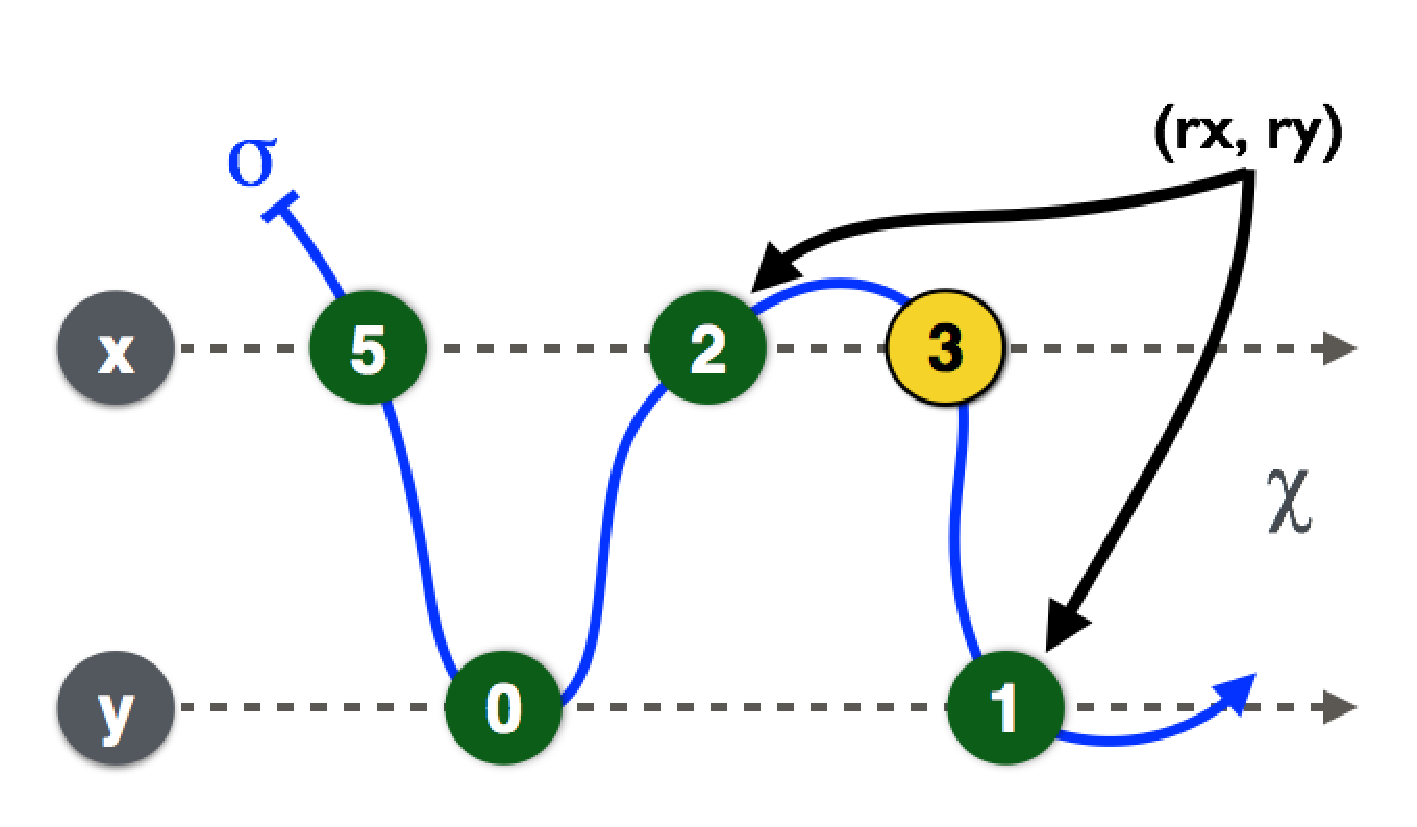
\includegraphics[width=6.1cm]{relink-before3.pdf}
\caption{\label{fig:reorder:before}} % Logical $=$ Real Time order, not a snapshot}
\end{subfigure} \hfill
\begin{subfigure}[t]{0.49\textwidth}
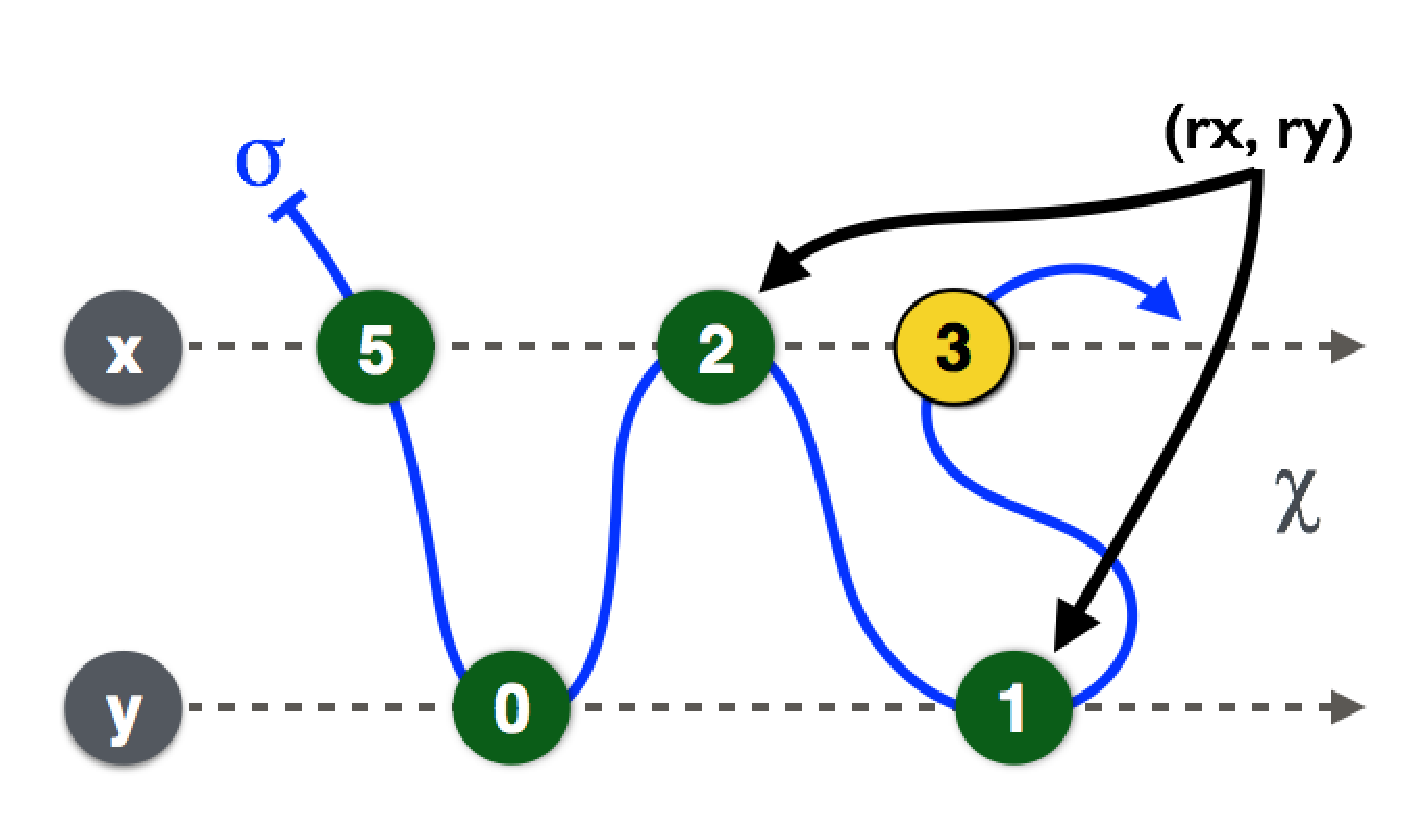
\includegraphics[width=6.1cm]{relink-after3.pdf}
\caption{\label{fig:reorder:after}} % Logical $\neq$ Real Time order, snapshot OK}
\end{subfigure}%
%
\caption{\label{fig:reorder} Changing the logical ordering (solid line
  $\ordlist$) of write events from (5, 0, 2, 3, 1) in
  (\subref{fig:reorder:before}) to (5, 0, 2, 1, 3) in
  (\subref{fig:reorder:after}), to reconcile with {\tt scan} returning
  the snapshot $\x=2, \y=1$, upon missing the write of $3$. Dashed
  lines $\hist$ represent real-time ordering.}
\end{figure}


Obviously, the high-level pattern of the proof requires tracking the
\emph{logical ordering} of the \jywrite\ and \jyscan\ events, which
differs from their \emph{real-time ordering}. As the logical ordering
is inherently dynamic, depending on properties such as
\jyscan\ missing a \jywrite, we formalize it in Hoare logic, by
keeping it as a list of events in auxiliary state that can be
dynamically reordered as needed. For example, Figure~\ref{fig:reorder}
shows the situation in the execution of \jyscan~that we reviewed
above. We start with the (initializing) writes of $5$ and $0$ already
executed, and our program performs the writes of $2$, $3$ and $1$ in
the real time order shown by the position of the events on the dashed
lines. In Figure~\ref{fig:reorder:before}, the logical order
$\ordlist$ coincides with real-time order, but is unsound for the
snapshot $\x=2, \y=1$ that \jyscan~wants to return. In that case, the
auxiliary code with which we annotate \jyscan, will change the
sequence $\ordlist$ in-place, as shown in
Figure~\ref{fig:reorder:after}.

Our specification and verification challenge then lies in reconciling
the following requirements. First, we have to posit specs that
say that \jywrite\ performs a write, and \jyscan\ performs a scan of
the memory, with the operations executing in a single logical
moment. Second, we need to implement the event reordering discipline
so that a method call only reorders events that overlap with it; the
logical order of the past events should be preserved. This will be
accomplished by introducing yet further structures into the auxiliary
state and code. Finally, the specs must hide the specifics of
the reordering discipline, which should be internal to the snapshot
object. Different snapshot implementations should be free to implement
different reorderings, without changing the method specs.


%Our challenge then lies in reconciling the following two conflicting
%requirements. First, we need to implement the reordering discipline so
%that the subsequent calls to \jywrite~and \jyscan~preserve the
%established logical order of the past events. This will be
%accomplished by introducing yet further structures into the auxiliary
%state and code. Second, we have to engineer Hoare triples for
%\jywrite~and \jyscan~to be \emph{intuitive} and \emph{helpful} to
%clients, but also to \emph{not expose} the specifics of the reordering
%discipline, which is internal to the snapshot object\footnotemark.
%%We discuss these issues next.
%\footnotetext{\ie we want to give the methods {\it principal} specifications}




\section{Outline of the mechanized development}
\label{sec:devel}

We next discuss how the above informal overview is mechanized in
Coq. We start with the definition of \code{span_tp} and proceed to
explain all of its components.
%
%At the level of using the tool, we illustrate how the power to
%combine proofs and programs enables building formal infrastructure for
%concurrent reasoning, such as concurroids and atomic actions. At the
%level of concurrency reasoning, we illustrate that our way of
%splitting the state into \emph{self}, \emph{joint} and \emph{other},
%leads to very simple and natural way to specify the various
%subcomponents that go into the implementation and proof of
%\code{span}. These two points together substantiate that FCSL
%abstractions are practically \emph{expressive} and can support
%straightforward specification and \emph{compositional} (\ie, divisible
%into libraries) and \emph{foundational} (\ie, from first principles)
%mechanized verification, of intricate programs that utilize
%\emph{realistic} fine-grained concurrent features.
%
The specifications and code shown will be very similar to what's in
our Coq files, though, to improve presentation, we occasionally take
liberties with the order of definitions and notational
abbreviations. We do not assume any familiarity with Coq, and explain
the code displays as they appear. We also omit the proofs and
occasional auxiliary definitions, which can be found in the FCSL code,
accompanying the paper.

\subsection{The definition of the type \texttt{span\_tp}}

The type \code{span_tp} is defined in Figure~\ref{fig:span_tp}.
%
It is an example of a \emph{dependent type}, as it takes formal
arguments in the form of variables \code{x}, \code{i} and \code{g1},
that the body of the type can use, \ie, \emph{depend on}.  The roles of
the variables differ depending on the keyword that binds them.
%
For example, the Coq keyword \code{forall} binds the variable \code{x}
of type \code{ptr}, and indicates that \code{span_tp} is a
specification for a procedure that has \code{x} as input. Indeed,
\code{span} is exactly such a procedure, as apparent from
Section~\ref{sec:overview}. Using \code{forall} to bind \code{x}
allows \code{x} to be used in the body of \code{span_tp}, \emph{but
  also in the body} of \code{span} (Figure~\ref{fig:coq-span}).
%
On the other hand, \code{i} and \code{g1} are bound by FCSL binder
\code{\{...\}}. This binding is different; it allows \code{i} and
\code{g1} to be used in the body of \code{span_tp}, \emph{but not in
  the procedure} \code{span}. In terminology of Hoare-style logic,
\code{i} and \code{g1} are \emph{logical variables}
(aka.~\emph{ghosts}), which are used in specs, but not in the code.
%
\code{STsep} is a Coq macro, defined by FCSL announcing that what
follows is a Hoare-style partial correctness specification for a
concurrent program. The component \code{SpanTree sp} in the brackets
is the concurroid whose protocol \code{span_tp} respects. We will
define \code{SpanTree} shortly. Finally, the parentheses
include the precondition and the postcondition (defined as Coq's
\code{fun}ctions) that we want to ascribe to \code{span}. The
precondition is a predicate over the pre-state \code{s1}. The
postcondition is a predicate over the boolean result \code{r} and
post-state \code{s2}. As customary in many programming languages, Coq
included, we omit the types of various variables when the system can
infer them (\eg, the variables \code{i}, \code{s1} and \code{s2} are
all of type \code{state}).

The precondition says that the input \code{x} is either \code{null}
(since \code{span} can be called on a leaf node), or belongs to the
domain of the input heap, and hence is a valid node in the
heap-represented graph. The heap is computed as the projection
\code{joint} out of the input state \code{s1}, which \code{i}
snapshots.  The projections \code{self} and \code{other} are sets of
marked nodes, belonging to the caller of \code{span} and to its
environment, respectively.

{\setlength{\belowcaptionskip}{-10pt} 
\begin{figure}[t!]
{\centering 
%[basicstyle=\footnotesize\ttfamily]
\begin{lstlisting}
Definition span_tp := forall (x : ptr),
  {i (g1 : graph (joint i))}, STsep [SpanTree sp] 
    (*  precondition predicate   *)
    (fun s1 => i = s1 /\ (x == null \/ x \in dom (joint s1)), 
    (*  postcondition predicate *)
     fun (r : bool) s2 => exists g2 : graph (joint s2), 
       subgraph g1 g2 /\ 
       if r then x != null /\ exists t,
         self s2 = self i \+ t /\ tree g2 x t /\ 
         maximal g2 t /\ front g1 t (self s2 \+ other s2)
       else (x == null \/ mark g2 x) /\ self s2 = self i). 
\end{lstlisting}
\vspace{-7pt}   
}
\caption{Specification \code{span_tp} of the \code{span} procedure.}
\label{fig:span_tp}
\end{figure}
}
%
The postcondition says that in the case the return result is \code{r =
  false}, the pointer \code{x} was either \code{null} or already
marked. Otherwise, there is a set of nodes \code{t} which is freshly
marked by the call to \code{span}; that is, \code{self s2} is a
\emph{disjoint union} (\code{\\+}) of \code{t} with the set of nodes
marked in the pre-state \code{self i}. The set \code{t} satisfies
several important properties.
%
First, \code{t} is a subtree in the graph, \Code{g2}, of the
post-state \code{s2}, with root \code{x}. Second, the tree \code{t} is
\emph{maximal}, \ie, it cannot be extended into a larger tree by
adding more nodes from \code{g2}, as all the edges between \code{t}
and the rest of the graph have been severed by \code{span}. Third, all
the nodes immediately reachable from \code{t} in the \emph{initial}
state \code{i} (\ie, \code{t}'s front) are marked in \code{g2} either
by this or some other thread (\code{self s2 \\+ other s2}). That is,
\code{span} did not leave any reachable nodes unmarked; if such nodes
existed, \code{span} would not have terminated.
%
Finally, in both cases, \code{subgraph g1 g2} states that the final
graph \code{g2} is obtained by marking nodes and removing edges from
the initial graph \code{g1}; no new edges are added, or nodes
unmarked.

We close the description of \code{span_tp} by noting its interesting
\emph{bi-directional} nature. It contains properties such as
\code{tree} and \code{maximal}, stated over the post-state graph
\code{g2} (forward direction), but also the property \code{front}
which is stated of the pre-state graph \code{g1}, and can be stated
only in relation to \code{s2} (backward
direction). The backward direction is a crucial component in the proof
that the top-most call to \code{span}, shielded from interference by
\textsf{hide}, indeed marked all the nodes and, hence, constructed a
tree, which spans the initial graph.

%The proof of this spec of the \code{span} program is about 200 LOC of
%Coq proof script, which is mostly dedicated to splitting
%\emph{self}-contributions between parallel threads and combining them
%upon their termination. Importantly, the specifications for recursive
%calls relate the initial/final graph \wrt the recursive calls
%themselves, but \emph{not} the initial/final graph of the enclosing
%call. This is why we need to reason in terms of forwards/backwards
%stability, described previously, to derive, in particular, the
%assertion about \code{front} at the \emph{end} \code{span}'s body from
%the postcondition of a recursive call to \code{loop}.

\subsection{Representing graphs in a heap}
Next we define the predicate \code{graph h}, which appears in
\code{span_tp} (Figure~\ref{fig:span_tp}), and says when a heap
\code{h} represents a graph. It does so if every pointer \code{x} in
\code{h} stores some triple \code{(b, xl, xr)}, where \code{b} is the
``marked'' bit, and \code{xl}, \code{xr} are pointers in the domain of
\code{h} (and, hence, are \code{x} itself or other nodes), or
\code{null} if \code{x} has no successors. 
%
\begin{lstlisting}
Definition graph (h : heap) := valid h /\ 
  forall x, x \in dom h -> exists (b : bool) (xl xr : ptr),
      h = x :-> (b, xl, xr) \+ free x h /\
      {subset [:: xl; xr] <= [:: null] ++ dom h}.   
\end{lstlisting}
%
The conjunct \code{valid h} says that the heap \code{h} doesn't contain duplicate
pointers. The notation \code{\\+} is overloaded and used for disjoint
union of sets of nodes in \code{span_tp}, and for disjoint union of
heaps in \code{graph}. In general, we use \code{\\+} for any PCM
$\pcmF$ operation.  \code{free x h} is the heap obtained by
deallocating \code{x} from \code{h}.  Finally, the last line is
concrete syntax for $\small{\{\mathtt{xl, xv}\} \subseteq \{\mathtt{null}\}
\cup \mathtt{dom\ h}}$.
%
%\an{Maybe remove \code{free x h} in favor of an extra heap variable.}

The \code{graph} predicate illustrates \emph{certified programming} in
Coq~\cite{Chlipala:BOOK}, \ie, the ability to use propositions as
types, and pass variables such as \code{g1} and \code{g2} that stand
for \emph{proofs} of the \code{graph} property, as inputs to other
types (\eg, \code{span_tp}) or functions. This ability enables
formally defining \emph{partial} functions over heaps that are
undefined when the heap doesn't encode a valid graph. An alternative
to this somewhat unique capability of dependent types, is to encode
partial functions as relations, but that usually results in increase
in proof tedium and size.

Here are a few examples of such partial functions. Given a node (\ie,
a pointer) \code{x} and a proof that the heap \code{h} represents a
graph (written (\code{g : graph h})), we name \code{mark g x},
\code{edgl g x} and \code{edgr g x} the three components stored in the
pointer \code{x} in the heap (\ie, the ``marked'' bit, left, right
successor), and write \code{contents g x} for the whole triple.  By
default, these values are \code{false}, \code{null}, \code{null} if
\code{x} is not in the heap.
%
Each of these functions takes \code{h} as an argument; \ie, one could
also write \code{mark h g x} \etc., but we omit \code{h} as it can be
inferred from \code{g}'s type, following Coq's standard notational
abbreviation.

We can now define the remaining predicates used in \code{span_tp} in
Figure~\ref{fig:span_tp}. For all of the definitions, we assume that variables
\code{h} and (\code{g : graph h}) are in scope, and omit them. We also use
\code{ptr_set} as an alias for finite maps from pointers to the unit
type.\footnote{This is a bit expedient way of implementing finite
  sets, but it saves work by reusing an extensive library of finite
  maps, also used for formalizing heaps.}

First, we define the function \code{edge}, representing the incidence
relation of the graph~\code{g}.

\begin{lstlisting}
Definition edge (x y : ptr) := 
  (x \in dom h) && (y != null) && (y \in [:: edgl g x; edgr g x]).
\end{lstlisting}

% (The last conjunct is Coq syntax for \code{y} is an element of the
%union of the two sets \code{edgl g x} and \code{edgr g x}.)
%\ab{Check.} \an{Erased the comment to save space. Up above we now
%discuss this notation a bit, so hopefully doing it once will suffice
%for the reader to orient herself here.}
Second, \code{tree x t} requires that \code{t} contains \code{x}, and
for any node \code{y}~$\in$~\code{t}, there exists a unique path (\ie,
a list of nodes) \code{p} from \code{x} to \code{y} via \code{edge}'s
links, which lies within the tree (\ie, the nodes \code{p} are a subset
of~\code{t}). Note how \code{edge} is \emph{curried}, \ie, passed to
\code{path} as a function, abstracted over arguments. This illustrates
that even simple mathematical mechanizations require higher-order
functions in order to~work.
%
\begin{lstlisting}
Definition tree (x : ptr) (t : ptr_set) := x \in dom t /\
  forall y, y \in dom t -> exists !p, 
    path edge x p /\ y = last x p /\ {subset p <= dom t}.   
\end{lstlisting} 
%
%
Third, \code{front\ t t'}, determines if the nodes reachable from
\code{t} in \emph{zero or one step} are included in \code{t'}.
%
\begin{lstlisting}
Definition front (t t' : ptr_set) :=
  {subset dom t <= dom t'} /\
  forall x y, x \in dom t -> edge x y -> y \in dom t'. 
\end{lstlisting}
%
Fourth, a tree \code{t} is maximal if it includes its front. A graph
is connected if there's a path from \code{x} to every other node in it.
\begin{lstlisting}
Definition maximal (t : ptr_set) := front t t.
Definition connected (x : ptr) (t : ptr_set) := forall y : ptr, 
  y \in dom t -> exists p, path edge x p /\ last x p = y.
\end{lstlisting}
%
Finally, \code{subgraph} codifies a number of properties between
pre-state \code{s1} and post-state \code{s2}, and their graphs
\code{g1}, \code{g2}. In particular: \code{g1}, \code{g2} contain the
same nodes (\code{=i} is equality on lists modulo permutation), the
set of self-marked and other-marked nodes only increase, edges out of
a node \code{y} can be changed only if the node is marked, and the
only change to the edges is nullification (that is, removal).
\begin{lstlisting}
Definition subgraph s1 s2 
  (g1 : graph (joint s1)) (g2 : graph (joint s2)) :=
  dom (joint s1) =i dom (joint s2) /\
  {subset dom (self s1) <= dom (self s2)} /\
  {subset dom (other s1) <= dom (other s2)} /\
  (forall y, ~~(mark g2 y) -> contents g1 y = contents g2 y) /\
  (forall x, (edgl g2 x \in [:: null; edgl g1 x]) /\
              (edgr g2 x \in [:: null; edgr g1 x])).
\end{lstlisting}

We close the description of the predicates used in \code{span_tp}, by
listing two important lemmas that relate them. The first lemma,
%
%\code{front_leq} lemma says that \code{front} is monotone \wrt its
%second argument. 
\code{max_tree2}, says that if \code{y1} and \code{y2} are
successors of \code{x} (\ie, \code{edge x} equals the set \code{[::
  y1; y2]} %\ab{Avoid the Coq syntax?} \an{Hmm. If I did it may be
% unclear what the syntax is refering to in the listing}
modulo permutation), and \code{ty1} and \code{ty2} are maximal trees
rooted in \code{y1} and \code{y2}, and moreover, \code{ty1} and
\code{ty2} are disjoint, then the set of nodes built from \code{x},
\code{ty1} and \code{ty2} by disjoint union (\code{\\+}) is a tree
itself, \ie, no edges connect \code{ty1} and \code{ty2} (the notation
\code{#x} is concrete syntax for the singleton finite map containing
node \code{x}).  This lemma is essential in proving that \code{span}
produces a tree, as mentioned in Section~\ref{sec:overview} for the
case $r_l\,{=}\,r_r\,{=}\,\mathtt{\small{true}}$.
%
%Lemma front_leq t t1 t2 : 
%  {subset dom t1 <= dom t2} -> front t t1 -> front t t2.
%
\begin{lstlisting}
Lemma max_tree2 x y1 y2 ty1 ty2 : 
  edge x =i [:: y1; y2] ->  tree y1 ty1 -> maximal ty1 ->
  tree y2 ty2 -> maximal ty2 -> valid (ty1 \+ ty2) -> 
  tree x (#x \+ ty1 \+ ty2).
\end{lstlisting}
The second lemma shows that \code{subgraph} is monotone \wrt~the
stepping of environment threads in the \code{SpanTree} concurroid.
%
\begin{lstlisting}
Lemma subgraph_steps s1 s2
  (g1 : graph (joint s1)) (g2 : graph (joint s2)) :
  env_steps (SpanTree sp) s1 s2 -> subgraph g1 g2.
\end{lstlisting}
We used this lemma as the main tool in establishing a number of
stability properties in Coq, related to the conjuncts from the
definition of \code{subgraph g1 g2}. For example, the lemma implies
that if \code{x} is a node of \code{joint s1}, then it is so in a
stable manner; that is, \code{x} is a node in \code{joint s2} for any
\code{s2} obtained from \code{s1}, by environment interference.

%property; that is, it holds of states \code{s1}, \code{s2}
%(and their graphs), if the concurroid can be moved from \code{s1} to
%\code{s2} by the environment threads (\ie, changing \emph{other}) in
%arbitrarily many steps.
%\ab{Unclear, rewrite this. \code{env\_steps} not defined. Perhaps want
%  to say that each of the conjuncts in \code{subgraph} implies a
%  stability property? The first one says \code{i} $\in$ \code{dom s1}
%  implies \code{i} $\in$ \code{dom s2}.}


\subsection{\texttt{SpanTree} concurroid}
\label{sec:graph-conc-coher}

% \todo{Rework this section in the same style as the actions one. That is: 
% (1) Say that the coherence predicate is essentially the state space. 
% (2) Go through some selected predicates in it, \eg, validH, validSO. 
% (3) Show how the transitions are formally implemented. No need to
% explain the intuition for them again, as that has already been given
% in the Overview section.
% (4) Say that our signatures require that a bunch of properties of
% transitions be proved, before an ordinary relation can be promoted
% to a transition. If some are chosen to be expanded on, make sure
% that they can be stated only in terms of concepts that have been
% introduced. In particular, it's not OK to use \code{\\<} and
% \code{\\>} without saying in more detail what they are, and perhaps
% even giving their formal definitions in terms of the PCM operations.
% (5) If no properties are chosen to be expanded on, just list some
% names for them informally, as was done for actions. Eg., just say
% that we have locality, frameability, invariance of other, etc. These
% names can be found in the appendix to the ESOP'14 paper. As in
% actions, these names will have some meaning to separation logic
% people. Decide to expand or not expand on some of the properties,
% depending on how much space we have. 
% (6) All of that said, we probably should not expand here, but use
% the space to expand on other sections, chiefly the description of
% getters.}

Next we define the \code{SpanTree} concurroid. Being an STS, the
definition includes the specification of the state space, and
transitions between states. In the case of concurroids, we have an
additional component: \emph{labels} (semantically, natural numbers)
that differentiate instances of the concurroid. Thus the
definition of \code{SpanTree} is parametrized by the variable
\code{sp}, which makes it possible to use several instances of
\code{SpanTree} with different labels in a specification of a single
program. For example, say we want to run two \code{span} procedures
in parallel on disjoint heaps. Such a program could be specified by a
Cartesian product of \code{SpanTree sp1} and \code{SpanTree sp2},
where the different labels \code{sp1} and \code{sp2} instantiate the
variable \code{sp}.

The state space of \code{SpanTree} is defined by the following state
predicate \code{coh}, which we call \emph{coherence predicate}.

%
%spanning tree concurroid \code{SpanTree} has already appeared in the
%specifications of the \code{trymark} action and the \code{span_tp}
%spec (Figure~\ref{fig:span_tp}) of \code{span}.
%%
%Its presence in the above types constrains the state space of
%the programs being specified by defining which states are
%considered to be \emph{coherent}, and what changes (\ie,
%\emph{transitions}) can be made in the resource by the interfering
%threads.
%
%A concurroid definition is parametrized by a \emph{label} (a natural
%number) \code{sp}, making it possible to use several of its instances
%with different labels in a single program (\eg, running two
%\code{span} procedures in parallel on disjoint heaps).
%%
%The state space is defined via the \emph{coherence} predicate
%\code{coh}:
%
\begin{lstlisting}
Variable sp : nat.
Definition coh s := exists g : graph (joint s), 
  s = sp ->> [self s, joint s, other s] /\ 
  valid (self s \+ other s) /\ 
  forall x, x \in dom (self s \+ other s) = mark g x.  
\end{lstlisting}
%
The coherence predicate codifies that the state \code{s} is a triple,
\code{[self s,} \code{joint s,} \code{other s]}, and that it is
labelled by \code{sp}. The proof \code{g} is a witness that the
\code{joint} component is a graph-shaped heap.
%
The conjunct \code{valid (self s \\+ other s)} says that the
\emph{self} and \emph{other} components of the auxiliary state are
disjoint; their union is a finite map which is \code{valid}, \ie,
doesn't contain duplicate keys.
%
The most important invariant is that a node \code{x} is contained in
either \emph{self} or \emph{other} subjective view \Iff it's marked in
the joint graph.
%
%In all of the previously shown specifications and action definitions,
%we implicitly assumed the subject state to be coherent in the sence of
%\code{coh}.

The metatheory of FCSL~\cite[\S4]{Nanevski-al:ESOP14} requires the
coherence predicates to satisfy several properties that we omit
here, but prove in our implementation. The most important property is
the \emph{fork-join closure}, stating that the state space is closed
under realignment of \emph{self} and \emph{other} components. In other
words, one may subtract a value from \emph{self} and add it to
\emph{other} (and vice versa), without changing the coherence of the
underlying state.

%As a requirement imposed by FCSL's metatheory
%soundness~\cite[\S4]{Nanevski-al:ESOP14}, a concurroid's coherence
%predicate should satisfy a number of properties: the validity of
%\emph{self} $\pcmF$ \emph{other} and of the captured heap, as well as
%\emph{fork-join closure}, stating that the state-space is closed under
%realignment of \emph{self} and \emph{other} (\ie, subtracting a part
%of a state from one and adding is to another, and vice versa).

%
\code{SpanTree sp} contains two non-idle transitions. Transition
\code{marknode_trans}, parametrized by the node \code{x}, 
describes how an unmarked \code{x} is physically marked in the joint
graph, and simultaneously added to the \emph{self} component.  The
transition \code{nullify_trans} is parametrized by node \code{x} and
the direction \code{c}, indicating the successor of \code{x} (left or
right) that must be cut off from the graph. We omit the definitions of the
functions \code{mark_node} and \code{null_edge} that describe the
physical changes performed by the two transitions to the underlying
shared graph. These can be found in the Coq code.
%
%
\begin{lstlisting}
Definition marknode_trans x s s' := exists g : graph (joint s),
 ~~(mark g x) /\ joint s' = mark_node g x /\
 self s' = #x \+ self s /\ other s' = other s /\ coh s /\ coh s'.  

Definition nullify_trans x (c : side) s s' := 
  exists g : graph (joint s), 
    x \in dom (self s) /\ joint s' = null_edge g c x /\
    self s' = self s /\ other s' = other s, coh s /\ coh s'.  
\end{lstlisting} 
%
% Marking a graph node \code{x}, described by the \code{marknode_trans}
% predicate, requires \code{x} to be not marked in the initial
% state~\code{s}; it also states that upon marking the node, a singleton
% set \code{#x} is joined to the self-component of the thread that
% initiated the transition, and that the node's marked bit is changed in
% the final joint heap~(\code{mark_node g x}).
%   
%  
% The \code{nullify} transition ensures that the node \code{x} is marked
% by the acting thread (\code{x \\in dom (self s)}) and removes a link
% to \code{x}'s successor (indicated by the direction~\code{c}, which is
% either \code{Left} or \code{Right}) in the final state \code{s'} via
% the function \code{null_edge}, which we omit.

The FCSL metatheory requires that transitions too satisfy several
properties. For example, \code{marknode_trans} and
\code{nullify_trans} preserve the \emph{other}-component and the
coherence predicate, as immediately apparent from their
definitions. They also preserve the footprint of the underlying state,
\ie, they don't add or remove any pointers. Adding and removing heap
parts can be accomplished by \emph{communication} between concurroids,
as we briefly discuss in Section~\ref{sec:more-examples}.

%The other properties to be proved for each of these transitions are:
%\emph{footprint preservation} (\ie, they don't alter the domain of the
%concurroid's heap) and \emph{locality}, which ensures that the
%transition can be ``framed''.\footnote{In FCSL, terminology both
%  \ccode{marknode_trans} nad \ccode{nullify-trans} are \emph{internal}
%  transitions, as they don't change the ownership over the heap. A
%  different class of \emph{external} transitions (with different
%  properties) serves for composing concurroids and is featured in
%  other exmaples.}

The coherence predicate, the transitions, and the proofs of their
properties, are packaged into a \emph{dependent record}\footnote{A
  type-theoretic variant of a C \ccode{struct}, where fields can
  contain proofs.} \code{SpanTree sp}, which encapsulates all that's
important about a concurroid. Thus, we use the power of dependent
types in an essential way to build mathematical abstractions, such as
concurroids, that are critical for reusing proofs.
%

% The coherence predicate and the transitions, together with the proofs
% of their properties, are used to instantiate the concurroid
% ``interface''.
% %
% % \footnote{Proofs are first-class values in Coq, so one can pass them
% %   as arguments.}
% %
% Such interface (omitted here for brevity) is implemented as Coq's
% \emph{dependent record}, so it ``packages'' the STS definition
% together with the proofs of its
% properties. Since the provided proofs
% become the values of the record's fields, they can be later extracted
% and employed in the reasoning about specific concurrent programs,
% operating with the defined concurroid.\footnote{\ccode{[Pred...]}-like
%   combinators construct predicates for generally undecidable
%   properties, \ie, those whose proofs should be explicitly
%   constructed.}
% %
% \begin{lstlisting}
% Canonical SpanCore : mod_core := 
%   Mod.Core [PredU [Pred r | exists x, r = marknode_trans x] & 
%                     [Pred r | exists x c, r = nullify_trans x c]].  
% Canonical SpanTree : mod := Mod.Make SpanCore Pred0.   
% \end{lstlisting}


\subsection{Atomic actions}
%
% \ab{This paragraph starts out well but becomes handwavy, due to lack
% of space.  Perhaps we should first write the paragraph on
% \Code{SpanTree} concurroid and then put Atomic action.}
%
We next illustrate the mechanism for defining atomic actions in FCSL.
The role of atomic actions is to perform a single physical memory
operation on the real heap, simultaneously with an arbitrary
modification of the auxiliary part of the state.
%Many related logics
%\ab{Citations} \an{Heh, gotta save space; PLDI format wastes a lot of space on citations.}
%
%specify these two different aspects of the atomic
%action as two separate operations. 
In FCSL, we treat the real and auxiliary state uniformly as they both
satisfy the same PCM laws. We specify their effects in one common
step, but afterwards prove a number of properties that separate
them. For instance, for each atomic action we always prove the
\emph{erasure property} that says that the effect of the action on the
auxiliary state doesn't affect the real state.

Specifically, the effect of the \code{trymark} action is defined by
the following relation between the input pointer \code{x}, the
pre-state \code{s1}, post-state \code{s2} and the return result
\code{r} of type \code{bool}.
%
\begin{lstlisting}
Definition trymark_step (x : ptr) s1 s2 (r : bool) := 
 exists g : graph (joint s1), 
   x \in dom (joint s1) /\ other s2 = other s1 /\ 
   if mark g x 
   then r = false /\ joint s2 = joint s1 /\ self s2 = self s1
   else r = true /\ joint s2 = mark_node g x /\ 
         self s2 = #x \+ self s1.
\end{lstlisting}
The relation requires that \code{x} is a node in the pre-state graph
(\code{x \\in dom (joint s1)}). If \code{x} is unmarked in this graph,
then the action returns \code{true}, together with marking the node
physically in the real state (employing the function \code{mark_node}
already used in \code{marknode_trans}). Otherwise, the state remains
unchanged, and the action's result is \code{false}.
%
Notice that when restricted to the real heap, \ie, if we ignore the
auxiliary state in \code{self s1} and \code{other s1}, the relation
essentially describes the effect of the \code{CAS} command on the mark
bit of \code{x}. Thus, \code{trymark} {\em erases} to \code{CAS}.

There are several other components that go into the definition of an
atomic action. In particular, one has to prove that transitions are
\emph{total}, \emph{local}, and \emph{frameable} in the sense of
Separation Logic, and then ascribe to each action a stable
specification. However, the most important aspect of action
definitions is to identify their behavior with some transition in the
underlying concurroid. For example, \code{trymark} behaves like
\code{marknode_trans} transition of \code{SpanTree} if it succeeds,
and like \code{idle} if it fails.  Actions may also change state of a
number of concurroids simultaneously, as we will discuss in
Section~\ref{sec:more-examples}.  In the interest of brevity, we omit
the formal definition of all these properties here, but they can be
found in the accompanying Coq files.

%\ab{The rest becomes handwavy.}  To fully define the
%action we also require a \emph{safety} predicate, which says when the
%action is safe to execute. For \code{trymark} we require that \code{x}
%be a node in the graph, so that \code{x} does in fact point to a
%``marked'' bit to perform a \code{CAS} on.
%%
%\begin{lstlisting}
%Definition trymark_safe (x : ptr) s := 
%  x \in dom (joint s) /\ graph (joint s).
%\end{lstlisting}
%%
%In addition to erasure property, our Coq signatures require a number
%of other properties to be proved for actions, such as \emph{totality},
%\emph{locality}, \emph{frameability},\footnote{In a sense similar to
%  that from separation logic~\cite{Reynolds:LICS02}.} adherence to the
%concurroid transitions, \etc. However, for brevity we omit these from
%the presentation.
%%
%Once all the properties are proved, the stepping relation, the safety
%relation, and the proofs of all the properties are packaged together
%into a \emph{dependent record},\footnote{A type-theoretic variant of a
%  C \ccode{struct}, where fields can contain proofs.} containing all
%that's important about the action~\cite{Garillot-al:TPHOL09}. In this
%case, the structure is called \code{trymark_act}.
%
%The final step in an action definition is to provide a \emph{Hoare
%  type} for it, in the style of \code{span_tp}, with a precondition
%and postcondition, which must be proven to be stable \wrt~the
%interference of the concurroid \code{SpanTree}. We list such a spec
%below, and note that the proof of the spec is conducted by weakening
%the action's safety and stepping relations in the spirit of explicit
%stabilization by~\citet{Wickerson-al:ESOP10}.
%%
%\begin{lstlisting}
%Program Definition trymark x :
%  {i (g1 : graph (joint i))}, STsep [SpanTree sp] 
%    (fun s1 => s1 = i /\ x \in dom (joint s1),
%     fun b s2 => exists (g2 : graph (joint s2)),
%       subgraph g1 g2 /\ mark g2 x = true /\
%       self s2 = (if b then #x \+ self i else self i) /\
%       b -> contents g1 x = (false, edgl g2 x, edgr g2 x))
%  := Do (act (trymark_act x)).  
%\end{lstlisting}
%%
%The precondition is stable because the set of nodes in the shared
%graph never changes (\eg, lemma \code{subgraph_steps}). Thus, if
%\code{x} is a node in the pre-state, it will be a node in any state
%that may be obtained by intereference from other threads.
%%
%The stability of the postcondition is more subtle. We only discuss the
%conjunct
%\begin{lstlisting}
%b -> contents g1 x = (false, edgl g2 x, edgr g2 x)
%\end{lstlisting}
%as it is the most interesting. This implication says that if the
%action succeeded (\ie, returned \code{b = true}), then the node
%\code{x} must have been unmarked in the initial graph \code{g1}, and
%had the same outgoing edges that \code{x} has in the ending graph
%\code{g2}. This property is stable for the following reasons.  Before
%\code{x} got marked, nobody could modify its edges, because the
%transitions of the concurroid \code{SpanTree} allow only edges from
%marked nodes to be removed, as we will later see in this section. Once
%\code{x} got marked, it became private to the calling thread, and thus
%no other threads could modify its edges.


\subsection{Scoped concurroid allocation and hiding}

The \code{span_tp} type from Figure~\ref{fig:span_tp} operates under
\emph{open-world assumption} that \code{span} runs in an environment
of interfering threads, which, however, respect the transitions of the
\code{SpanTree} concurroid. If one wants to protect \code{span} from
interference, and move to \emph{closed-world assumption}, the top-most
call must be enclosed within $\mathsf{hide}$. We next show how to
formally do so.

The $\mathsf{hide}$ construct allocates a new lexically-scoped
concurroid from a local state of a particular thread.\footnote{The
  thread-local state is modelled in FCSL by a basic concurroid
  \ccode{Priv pv} with a label
  \ccode{pv}~\cite[\S4]{Nanevski-al:ESOP14}. \ccode{Priv}'s self/other
  components are retrieved via \ccode{pv_self} and \ccode{pv_other} projections. }
%
% Therefore, all locally-spawned threads can interfere on the state,
% described by this concurroid, while it's ``hidden'' from any external
% thread.
%
The description of how much local heap should be ``donated'' to the
concurroid creation is provided by the user-supplied predicate $\Phi$,
called \emph{decoration} predicate. In addition to the heap, the
predicate scopes over the auxiliary \emph{self} value, while the
auxiliary \emph{other} is fixed to the PCM unit, to signal that
there's no interference from outside threads. In the case of
\code{span}, the decoration predicate is as follows.
%
\begin{lstlisting}
Definition graph_dec sp (g : heap * ptr_set) s := 
  exists (pf : graph g.1), s = sp ->> [g.2, g.1, Unit] /\ coh s. 
\end{lstlisting}
%Canonical SpanDecorate sp := Decorate (graph_dec sp) SpanTree.
%
%Coq's \code{Canonical} keyword~\cite{Mahboubi-Tassi:ITP13} registers
%the instance \code{SpanDecorate} of the interface \code{Decorate} with
%the specific predicate \code{graph_dec} to be the ``default one" for
%the role of annotation~$\Phi$ (Section~\ref{sec:overview}), used by
%Coq whenever it requires to allocate a concurroid of the kind
%\code{SpanTree}. A decoration predicate has to satisfy a number of
%properties such as \emph{precision} in the sense of Separation logic,
%but we omit these here.
%
%Together with the proofs of its properties (such
%as \emph{precision}, \emph{injectivity}, and \emph{surjectivity}), a
%decorator is used to instantiate the \code{Decorate} interface.

We can now write out a new type \code{span_root_tp}, to specify the
top-most call to \code{span}, under the closed-world assumption that
there's no interference. Parametrizing \wrt~the locally-scoped
variable \code{h1 : heap} that snapshots the initial heap, the type is
the following one.
%
\begin{lstlisting}
Definition span_root_tp (x : ptr) :=
  {g1 : graph h1}, STsep [Priv pv] 
    (* precondition predicate *)
    (fun s1 => (forall y, ~~ (mark g1 y)) /\
       pv_self s1 = h1 /\ x \in dom h1 /\ connected g1 x, 
    (* postcondition predicate *)
     fun (_ : bool) s2 => exists (g2 : graph (pv_self s2)) t, 
       (forall x, (edgl g2 x \in [:: null; edgl g1 x]) /\
                   (edgr g2 x \in [:: null; edgr g1 x])) /\
       tree g2 x t /\ dom t =i dom h1).
\end{lstlisting}
The precondition says that the argument \code{x} is the root of the
graph \code{g1} stored in \code{h1}, and all the nodes of \code{g1}
are reachable from \code{x}. 
%
The postcondition says that the final heap's topology is a tree
\code{t}, whose edges are a subset of the edges of \code{g1}, but
whose nodes include \emph{all} the nodes of \code{g1}. Thus, the tree
is a spanning one.
%
The program satisfying this spec is a call to \code{span}, wrapped
into $\mathsf{hide}$, annotated with the decorating functions. We also
supply \code{h1} as the initial heap, and \code{Unit} of the PCM of
finite sets (hence, the empty set), as the initial value for
\emph{self}, which indicates that \code{span} is invoked with the
empty set of marked nodes.
% 
\begin{lstlisting}
Program Definition span_root x : span_root_tp x := 
  Do (priv_hide pv (graph_dec sp) (h1, Unit) [span sp x]).  
\end{lstlisting}
%
Coq will emit a proof obligation that the pre and post of
\code{span_tp} can be weakened into those of \code{span_root_tp} under
the closed-world assumption that \code{other s2 = Unit}. This proof is
in the development, accompanying this paper.

\section{More examples}
\label{sec:more-examples}

We next briefly illustrate two additional features of FCSL that our
implementation uses extensively: concurroid composition and reasoning
about higher-order concurrent structures with work stealing.

\subsection{Composing concurrent resources}
\label{sec:comp-conc-reso}

The \code{span} algorithm uses only one concurroid \code{SpanTree},
allocated by $\mathsf{hide}$ out of the concurroid \code{Priv} for
thread-local state.
%
In general, FCSL specs can span multiple primitive concurroids, of the
same or different kinds, which are \emph{entangled} by interconnecting
special \emph{channel}-like transitions~\cite{Nanevski-al:ESOP14}. The interconnection
implements synchronized communication, by which concurroids 
exchange heap ownership.
%
Entangling several concurroids yields a new concurroid.
%
Omitting the formal details of the entanglement
operators, let us demonstrate a program
whose spec uses a composite concurroid.
%
\begin{lstlisting}
Definition alloc : {h : heap}, STsep [entangle (Priv pv) ALock] 
   (fun s1 => pv_self s1 = h, 
    fun r s2 => exists B (v : B), pv_self s2 = r :-> v \+ h) := 
  ffix (fun (loop : unit -> alloc_tp) (_ : unit) =>
    Do (res <-- try_alloc; 
        if res is Some r then ret r else loop tt)) tt.  
\end{lstlisting}
%
The \code{alloc} procedure implements a pointer allocator. Its
postcondition says that the initial heap \code{h} is augmented by a
new pointer \code{r} storing some value \code{v} (\code{r :-> v}). The
heap \code{h} is part of the \code{Priv} concurroid, as evident by the
projection \code{pv_self} in the precondition. The pointer \code{r} is
logically transferred from the concurroid \code{ALock} which
implements a coarse-grained (\ie, lock-protected) concurrent
allocator. Hence, the whole procedure \code{alloc} uses the composed
concurroid \code{[entangle (Priv pv) ALock]}.
%
The body of \code{alloc} implements a simple spin-loop, trying to
acquire the pointer by invoking the \code{try_alloc} procedure, omitted
here.

Whereas separation logic~\cite{Reynolds:LICS02} always assumes
allocation as a primitive operation, the above example illustrates
that in FCSL, allocation is definable. One can also define a new
variant of the \code{STsep} type that automatically entangles the
underlying concurroid with \code{ALock}, thus enabling allocation
without the user having to explicitly do so herself.

\subsection{Higher-order specifications}
\label{sec:high-order-spec}

Due to embedding in Coq, FCSL is also capable of specifying and
verifying higher-order concurrent data structures, which we illustrate
by an example of a universal non-blocking construction of \emph{flat
  combining} by~\citet{Hendler-al:SPAA10}.\footnote{For simplicity, we
  present here a specification that is much weaker than what we have
  actually verified in our implementation.}

A flat combiner (FC) is a higher-order structure, whose method
\code{flat_combine} takes a sequential state-modifying
function~\code{f} and its argument~\code{v}, and works as
follows. While for the client, invoking \code{flat_combine(f, v)} looks
like a sequence \texttt{\small{lock; f(v); unlock}}, in reality, the
structure implements a sophisticated concurrent
behavior. Instead of expensive locking and unlocking, the calling
thread doesn't run \code{f}, but only \emph{registers} \code{f} to be
executed on \code{v}. One of the threads then becomes a
\emph{combiner} and executes the registered methods on behalf of
everyone else. Since only the combiner needs exclusive access to the
data structure, this reduces contention and improves cache
locality. This design pattern is known as \emph{work stealing} or
\emph{helping}: a thread can complete its task even without accessing
the shared resource.

To specify FC, we parametrize it by a sequential data structure and a
\emph{validity predicate} \code{fc_R}, which relates a function
\code{f} (from a fixed set of allowed operation), the argument of type
\code{fc_inT f}, result of type \code{fc_outT f} and the
\emph{contribution} of type \code{fc_pcm}. The last entry is a
description of what \code{f} \emph{does} to the shared state,
expressed in abstract algebraic terms as a value from a user-supplied
PCM.
%
\begin{lstlisting}
Variable fc_R : forall f, fc_inT f -> fc_outT f -> fc_pcm -> Prop.
\end{lstlisting}
%
The spec of the \code{flat_combine} is then given in the context of
three entangled concurroids: \code{Priv} for thread-local state, a
lock-based allocator \code{Alloc}, adapted from the previous example
(since a sequential function \code{f} might allocate new memory), and
a separate concurroid \code{FlatCombine}.
%
\begin{lstlisting}
Definition PA := (entangle (Priv pv) Alloc).
Definition W  := (entangle PA (FlatCombine fc)).  
Program Definition flat_combine f (v : fc_inT f) : STsep [W] 
 (fun s1 => pv_self s1 = Unit /\ fc_self s1 = Unit,
  fun (w : fc_outT f) s2 => exists g,
     pv_self s2 = Unit /\ fc_self s2 = g /\ fc_R f v w g) := ...
\end{lstlisting}
% 
The precondition says that \code{flat_combine} executes in the empty
initial heap (which is encoded as \code{pv_self s1 = Unit}), and hence
by framing, in any initial heap. Similarly, the initially assumed
effects of the calling thread on the shared data structure are empty
(\code{fc_self s1 = Unit}), but can be made arbitrary by applying
FCSL's \emph{frame rule} to the spec of \code{flat_combine}.
%
The postcondition says that there exists an abstract PCM value
\code{g} describing the effect of \code{f} in terms of PCM elements
(\code{fc_R f v w g}). Moreover, the effect of \code{g} is attributed
to the invoking thread (\code{fc_self s2 = g}), even though in reality
\code{f} could be executed by the combiner, \emph{on behalf} of the
calling thread.
%
In our Coq implementation, we instantiated the FC structure with a sequential
stack, showing that the result has the same spec as a concurrent stack
implementation.


\section{Elements of FCSL infrastructure}
\label{sec:underhood}

In this section we sketch two important parts of FCSL machinery, used
to simplify construction of proofs.

\subsection{Extracting concurroid structure via getters}
\label{sec:getters}

When working with compositions of multiple concurroids, as in examples
listed in Section~\ref{sec:more-examples}, one frequently has to
select the \emph{self}, \emph{joint} or \emph{other} components that
belong to one of the composed concurroids. A na\"{i}ve way of doing this
is to describe the state space of the composition concurroid using 
existentials that abstract over the concurroid-specific
fields. \emph{E.g.}, in the case of flat combiner, which composes
three concurroids \code{Priv}, \code{Alloc} and \code{FlatCombine}, we
could use three existentials to abstract over
\emph{self}/\emph{joint}/\emph{other} fields for \code{Priv}, another
three for \code{Alloc}, and three more for \code{FlatCombine}. To access
any of the fields, we have to destruct all
nine of the existentials. This quickly becomes tedious and results in
proofs that are obscured by such existential destruction.

Our alternative approach develops a systematic way of projecting the
fields associated with each concurroid, based on the concurroid's
label. Thus, for example, we can write \code{self\ pv\ s} to obtain
the \emph{self} component of \code{s}, associated with a concurroid
whose label is \code{pv}. The identifier \code{pv_self} we used in the
spec for \code{span_root} and for \code{flat_combine} is a notational
abbreviation for exactly this projection. While this is a simple and
obvious idea, its execution required a somewhat involved use of
dependently-typed programming, and an intricate automation by
canonical structures and lemma
overloading~\cite{Gonthier-al:ICFP11,Mahboubi-Tassi:ITP13}.

%As it was shown in Section~\ref{sec:more-examples}, most of the
%programs ``span'' a set of resources, described by a composite
%concurroid. To make proofs in such cases as simple as proofs about
%primitive (one-label) concurroids, we used the power of
%dependently-typed programming and implemented a library of \emph{state
%  getters}.
%
%Given the label of an arbitrary primitive concurroid, the type of its
%self/other and the joint component (which is typically \code{heap}),
%and the default value for the joint component, the function
%\code{Getter} will provide a dependent record with the three getters
%for this concurroid's state components.
%
%The following code shows an instantiation of the \code{Getter}
%interface for the graph concurroid, with a label \code{sp}, auxiliary
%state's type \code{ptr_set} and joint component to be a heap.
%
%\begin{lstlisting}
%Notation ptr_set := (ptrmap_pcm_Encoded [encoded_set of unit]).  
%Definition spg := Getter sp ptr_set heap_tp_Encoded Unit.
%
%Notation self s := (self spg s).
%Notation other s := (other spg s). 
%Notation joint s := (joint spg s).
%\end{lstlisting}

\subsection{Structural lemmas}
\label{sec:lemmas}

The proofs in FCSL are structured to facilitate systematic application
of Floyd-style structural rules, one for each program command. All the
rules are proved sound from first principles, and are applied as
lemmas to advance the verification.
%
As the first step of every proof, the system implicitly applies the
weakening rule to the automatically synthesized weakest pre- and
strongest postconditions~\cite{Dijkstra:CACM75}, essentially
converting the program into the continuation-passing style (CPS)
representation and sequentializing its structure.
%
Every statement-specific structural rule ``symbolically evaluates''
the program by one step, and replaces the goal with a new one to be
verified.

For example, the following lemma \code{step}, corresponding to the
rule of sequential composition, reduces the verification of a program
$(y \asgn e_1; (e_2~y))$ with continuation~$k$, to the verification
of the program $e_1$ and the program $e_2~y~k$, where $y$ corresponds
to a symbolic result of evaluating $e_1$, constrained according to
$e_1$'s postcondition. One can apply it several times until $e_1$ is
reduced to some primitive action, at which point one can apply the
structural rule for that action.
%
\begin{lstlisting}
Lemma step W A B (e1 : ST W A) (e2 : A -> ST W B) i (k : cont B): 
     verify i e1 (fun y m => verify m (e2 y) k) -> 
     verify i (y <-- e1; e2 y) k.  
\end{lstlisting}
%
\code{ST} is a type synonym for \code{STsep}, hiding its pre- and
postconditions.






\section{Mechanization and Evaluation}
\label{sec:evaluation}

% \ab{This is an important section. It needs to convey what was
%   difficult, what was easy in the implementation. How were the
%   difficulties mitigated via the techniques developed in the previous
%   sections? What interesting proof engineering that needed to be done?
%   Ideally, these discussions should provide context/understanding of
%   the numbers in the Table. What are the current limitations of the
%   implementation? Make a separate paragraph for limitations perhaps
%   starting ``At the moment'' below.}
%
% \is{Mostly addressed in revised writing.}

In order to assess feasibility of the presented above ideas, we have
mechanized the specs and the proofs of all the examples from this
paper, taking advantage of the fact that FCSL has been recently
implemented as a tool for concurrency
verification~\cite{Sergey-al:PLDI15} on top of the Coq proof
assistant~\cite{Coq-manual}.

Table~\ref{tab:locs} summarizes the statistics with respect to our
mechanization in terms of lines of code and compilation times. 
%
The examples were proof-checked on a 3.1~GHz Intel Core~i7 OS~X
machine with 16 Gb RAM, using Coq~8.5pl2 and Ssreflect
1.6~\cite{Gonthier-al:TR}.
%
As the table indicates, a large fraction of the implementation is
dedicated to proofs of preservation of resource
invariants~(\textsf{Inv}), \ie, checking that the actual
implementations do not ``go wrong''.
%
In our experience, these parts of the development are the most tricky,
as they require library-specific insights to define and reason about
auxiliary histories.
%
Since FCSL is a general-purpose verification framework, which does not
target any specific class of programs or properties, we had to prove
problem-specific facts, \eg, lemmas about histories of a particular
kind (\textsf{Facts}), and to establish the specs of interest stable
(\textsf{Stab}). Once this infrastructure has been developed, the
proofs of main procedures turned out to be relatively small
(\textsf{Main}).
%
% \gad{I don't see the point of having the {\bf Build} column in
%   Table~\ref{tab:locs}: First of all, I don't think that time to
%   compile a proof in Coq is relevant at all. From an engineering
%   perspective, it might perhaps make more sense to estimate the amount
%   of man-hours that took to discharge them. Second, because we then
%   would have to explain why the exchanger takes half the time than the
%   counter, given that they are similar in size. And I don't think we
%   want to get into describing the design, the differences in ``style''
%   between the two, and discussing why that might be affecting the
%   buildtime in detail here.}
%
% \is{Sorry, but since it's PLDI, we have to give build times, even
%   though we're out of space to explain some specific performance
%   phenomena}

{
%\setlength{\belowcaptionskip}{-1pt} 
\begin{table}
{%\footnotesize
\sffamily\small % tabular data either 10pt times, or 9pt helvetica
\centering
\begin{tabular}{|@{\ }l@{\ }||@{\ }c@{\ }|@{\ }c@{\ }|@{\ }c@{\ }|@{\ }c@{\ }|@{\ }c@{\ }||@{\ }r@{\ }|}
  \hline
  \textbf{Program} &  
                     {Facts} & {Inv} &
                                       {Stab} & {Main} & \textbf{Total}
  & \textbf{Build~~~}    
  \\ \hline \hline 
  Exchanger \hfill (\S \ref{sec:exchanger}) & 365 & 1085 & 446 & 162 & 2058 & 4m~~46s
  \\
  Exch. Client \hfill (\S \ref{sec:cal}) & 258 & -- &--& 182 & 440 & 57s
  \\
  Count. Netw. \hfill (\S \ref{sec:counting}) & 379 & 785 & 688 & 27 & 1879 & 12m~23s
  \\
  CN Client 1 \hfill (\S \ref{sec:qc-client}) & 141 &--&--& 180  & 321 & 3m~11s
  \\
  CN Client 2 \hfill (\S \ref{sec:qqc-client})& 115 &--&--& 259 & 374 & 3m~~~9s 
  \\[2pt] \hline
\end{tabular}
}
\caption{
  Mechanization of the examples: lines of code for program-specific facts \intab{Facts},
  resource invariants and transitions \intab{Inv}, 
  stability proofs for desired specs \intab{Stab}, spec and proof sizes for main
  functions \intab{Main}, total LOC count \intab{\textbf{Total}}, and build
  times \intab{\textbf{Build}}. The ``--'' entries indicate the
  components that were not needed for the example.
} 
\label{tab:locs}
%\vspace{-15pt}
\end{table}}

Fortunately, trickiness in libraries is invisible to clients, as FCSL
proofs are compositional. Indeed, because specs are encoded as Coq
types~\cite{Sergey-al:PLDI15}, the substitution principle
automatically applies to programs \emph{and proofs}.
%
%Thus, the trickiness of library proofs is not visible to the clients.
%
At the moment, our goal was not to optimize the proof sizes, but to
demonstrate that FCSL as a tool is suitable \emph{off-the-shelf} for
machine-checked verification of properties in the spirit of novel
correctness
conditions~\cite{Hemed-al:DISC15,Aspnes-al:JACM94,Jagadeesan-Riely:ICALP14}.
Therefore, we didn't invest into building advanced
tactics~\cite{McCreight:TPHOL09} for specific classes of
programs~\cite{Zee-al:PLDI08} or
properties~\cite{Dragoi-al:CAV13,Vafeiadis:CAV10,Bouajjani-al:POPL15,Burckhardt-al:PLDI10},
and we leave developing such automation for future work.

% Our verification is compositional, because the proofs of the clients'
% specs are derived only from the specifications of concurrent objects,
% without relying on their implementation.



\section{Related Work}
\label{sec:related}

% Existing methods for specifying the behavior of concurrent data
% structures and programs are either history-based or state-based.
% %
% The former ones describe the behavior of an object by describing and
% characterizing call/return strings that can be obtained by invoking
% the methods concurrently by several threads. 
% %
% The later ones define the object's behavior by posing requirements to
% a state, in which object's methods are safe to run, and stating
% assertions over a state, resulting from the object's method call. The
% second group of approaches employs program logics as a way to specify
% the state of interest as well as a mechanism to compose the program
% specifications.

% This paper contributes to the goal of unifying the history- and
% state-based views to specification and verification of concurrent
% objects.

% In this section we describe related approaches for reasoning about
% concurrency that have motivated our work.

\paragraph{Linearizability and history-based criteria.}

% In the past 25 years, linearizability has been widely applied to
% capture the behavior of concurrent objects with intuitive sequential
% specifications, and even suitable for automatic synthesis of some
% concurrent objects~\cite{Vechev-Yahav:PLDI08}. Thanks to the
% compositional proof method, based on \emph{linearization points},
% proofs of linearizability in most of the cases are amenable for
% practical computer-aided
% verification~\cite{Burckhardt-al:PLDI10,Derrick-al:TOPLAS11,Vafeiadis:CAV10,Amit-al:CAV07,Shacham-al:OOPSLA11,Dragoi-al:CAV13}.

The need for correctness criteria alternative to
linearizability~\cite{Herlihy-Wing:TOPLAS90}, which is more relaxed
yet compositional, was recognized in the work on counting
networks~\cite{Aspnes-al:JACM94}.
%
The suggested notion of quiescent
consistency~\cite{Shavit-Zemah:TOPLAS96} required the operations
separated by a quiescent state to take effect in their logical order.
%
%
A more refined correctness condition, \emph{quasi-linearizability},
implementing a relaxed version of linearizability with an upper bound
on nondeterminism, was proposed by Afek~\etal~\cite{Afek-al:OPODIS10},
allowing them to obtain the quantitative boundaries similar to what we
proved in Section~\ref{sec:qqc-client}.
%
The idea of relaxed linearizability was later used in the work on
\emph{quantitative relaxation} (QR)~\cite{Henzinger-al:POPL13} for
designing scalable concurrent data structures by changing the
specification set of sequential histories.
%
Most recently, \emph{quantitative quiescent consistency} has been
proposed as another criterion incorporating the possibility to reason
about effects of bounded thread
interference~\cite{Jagadeesan-Riely:ICALP14}.
%
It is worth noticing that some of these correctness criteria are
incomparable (\eg, QC and QR~\cite{Henzinger-al:POPL13}, QL and
QQC~\cite{Jagadeesan-Riely:ICALP14}) hence, for a particular
concurrent object, choosing one or another criterion should be
justified by the needs of the object's client. Therefore, a suitable
correctness condition is essentially ``\emph{in the eye of the
  beholder}'', as is typical in programming, when designing libraries
and abstract data structures, and the logic-based approach we advocate
provides precisely this flexibility in choosing desired specs.

% However, how suitable is one or another relaxed correctness
% condition %from the listed ones
% for reasoning about safety properties of a particular client program
% is still largely an open question.

\paragraph{Hoare-style specifications of concurrent objects.}
\label{sec:related-logic-based}

% Program logics for concurrency allow one to capture in the
% specification precisely those bits of information about the program's
% state, which are relevant for the program's clients, making it
% possible to abstract over the irrelevant details of the
% implementation~\cite{DinsdaleYoung-al:ECOOP10}.

Hoare-style program logics were used with great success to verify a
number of concurrent data structures and algorithms, which are much
more natural to specify in terms of observable state modifications,
rather than via call/return histories. The examples of such objects
and programs include
barriers~\cite{Dodds-al:POPL11,Hobor-Gherghina:ESOP11}, concurrent
indices~\cite{ArrozPincho-al:OOPSLA11}, flat
combiner~\cite{Turon-al:ICFP13,Sergey-al:ESOP15}, event
handlers~\cite{Svendsen-Birkedal:ESOP14}, shared graph
manipulations~\cite{Raad-al:ESOP15,Sergey-al:PLDI15}, as well as their
multiple client programs.
%
The observation about a possibility of using program logics as a
correctness criterion, alternative to linearizability, has been made
in some of the prior
works~\cite{Jacobs-Piessens:POPL11,ArrozPincho-al:OOPSLA11,Svendsen-al:ESOP13}.
%
Their criticism of linearizability addressed its inability to capture
the state-based properties, such as dynamic memory
ownership~\cite{Jacobs-Piessens:POPL11}---something that
linearizability indeed cannot tackle, unless it's
extended~\cite{Gotsman-Yang:CONCUR12}.
%
However, we are not aware of any prior attempts to capture CAL, QC and
QQC-like properties of concurrent executions by means of \emph{one and
  the same} program logic and employ them in client-side
reasoning.

%
% Verification in such logics is done structurally, \ie, by
% systematically applying syntax-directed inference rules, until the
% spec is proved. Several mechanized tools for logic-based
% concurrent reasoning have been
% released~\cite{Sergey-al:PLDI15,Appel-al:BOOK14}.

Several logics for proving linearizability or, equivalently,
observational refinement~\cite{Filipovic-al:TCS10,Turon-al:POPL13},
have been proposed
recently~\cite{Turon-al:ICFP13,Liang-Feng:PLDI13,Vafeiadis:PhD}, all
employing variations of the idea of using \emph{specifications as
  resources}, and identifying (possibly, non-fixed or non-local)
linearization points, at which such specification should be ``run''.
%
In these logics, after establishing linearizability of an operation,
one must still devise its Hoare-style spec, such that the spec is useful for
the clients.
% %
% To avoid this detour, a number of other logic-based approaches have
% suggested to assign Hoare-style specifications \emph{directly} to
% fine-grained object
% implementations~\cite{Svendsen-al:ESOP13,Svendsen-Birkedal:ESOP14,ArrozPincho-al:ECOOP14}
% and reason out of these specs.

Similarly to the way linearizability allows one to replace a
concurrent operation by an atomic one, several logics have implemented
the notion of \emph{logical atomicity}, allowing the clients of a data
structure to implement application-specific synchronization on top of
the data structure operations.
%
Logical atomicity can be implemented either by parametrizing specs
with client-specific auxiliary
code~\cite{Jacobs-Piessens:POPL11,Svendsen-al:ESOP13,Svendsen-Birkedal:ESOP14,Jung-al:POPL15}
or by engineering dedicated rules relying on the simulation between
the actual implementation and the ``atomic''
one~\cite{ArrozPincho-al:ECOOP14}.
%
% Both approaches to logical atomicity require one to identify precisely
% a \emph{synchronization point}~\cite{Svendsen-al:ESOP13} within the
% structure being verified, which makes it non-trivial to apply them for
% specifying non-linearizable objects, especially when conducting
% quantitative logic-based reasoning, which we demonstrated in
% Section~\ref{sec:qqc-client}.

Instead of trying to extend the existing approaches for logical
atomicity to non-linearizable objects (for which the notion of
atomicity is not intuitive), we relied on a general mechanism of
auxiliary state, provided by FCSL~\cite{Nanevski-al:ESOP14}. 
%
Specifically, we adopted the idea of histories as auxiliary
state~\cite{Sergey-al:ESOP15}, which, however, was previously explored
in the context of FCSL only for specifying linearizable structures.
%
% Similarly to logical atomicity, the histories-as-state specification
% approach makes fine-grained concurrent programs look like atomic ones,
% since due to compositionality, the specification clients only see the
% history entries.
%
% 
We introduced enhanced notation for referring directly to histories
(\eg, $\hists$, $\histo$), although FCSL's initial logical
infrastructure and inference rules remained unchanged.

% Recently, attempts were made to unify the common idioms occurring in a
% number of concurrency logics in a generic framework of
% \emph{Views}~\cite{DinsdaleYoung-al:POPL13}.
% %
% However, that result is orthogonal to our findings, as \emph{Views}
% are a framework for proving logics sound, not to prove programs, and
% this paper, we focused on using a particular logic (FCSL) for specifying a
% new class of concurrent data structures.
The purpose of \emph{Views}~\cite{DinsdaleYoung-al:POPL13} is to provide a PCM-based semantic framework for proving soundness of logics and type systems, and thus to unify common idioms occurring in several recent concurrency logics. However, the framework has not used PCMs for auxiliary state and/or specification of user programs. \ab{Please check.}


In this work, we do not argue that FCSL is the only logic capable of
encoding custom correctness conditions and their combinations, though,
we are not aware of any other work exploring a similar possibility.
%
However, we believe that FCSL's explicit \emph{other}
subjective state component provides the most straightforward way to do
so.
%
The logics like CAP~\cite{DinsdaleYoung-al:ECOOP10} and
TaDA~\cite{ArrozPincho-al:ECOOP14}, from our experience and personal
communication with their authors, may be capable of implementing our
approach at the expense of engineering a much more complicated
structure of capabilities to encode histories and their invariants,
and ``snapshot'' interference of an environment.
%
Other logics incorporating the generic PCM
structure~\cite{Raad-al:ESOP15,Jung-al:POPL15,Jung-al:ICFP16,Turon-al:OOPSLA14}
might be able to implement our approach, although none of these logics
provide an FCSL-style rule for hiding~\eqref{eq:ehide} as a uniform
mechanism to express explicit quiescence.

%\todo{State that in our cases histories are per-object.}

Concurrently with this work, Hemed~\etal developed a (not yet
mechanized) verification technique for CAL~\cite{Hemed-al:DISC15},
which they applied to the exchanger and the elimination
stack. Similarly to our proposal, they specify CAL-objects via Hoare
logic, but using one global auxiliary history, rather than subjective
auxiliary state. 
%
This tailors their system specifically to CAL (without a possibility
to incorporate reasoning about other, non CA-linearizable, concurrent
structures), and to programs with a \emph{fixed} number of threads. In
contrast, FCSL supports dynamic thread creation, and is capable of
uniformly expressing and mechanically verifying several different
criteria, with CAL merely a special case, obtained by a special choice
of PCM. Moreover, in FCSL the criteria combine, as illustrated in
Section~\ref{sec:cal}, where we combined quiescence with CAL via
hiding. Hiding is crucial for verifying clients with explicit
concurrency, but is currently unsupported by Hemed~\etal's method.
%
% Related is the property of our histories that no event may appear
% between two twin timestamps. We used this property to verify the
% client in Section~\ref{sec:cal}, but this does not seem to hold for
% histories used by Hemed~\etal

%Concurrently with our work, Hemed~\etal developed a (not yet
%mechanized) verification technique for
%CAL~\cite{Hemed-al:DISC15}. Similarly to our proposal, they employed
%the idea of specifying CAL-objects via Hoare triples with auxiliary
%histories. Unlike our approach, their choice of abstractions is
%tailored for conducting proofs about CAL, and they don't establish a
%soundness result of their Hoare-style specs, with respect to CAL or
%any other semantics. In contrast, what we propose is using a uniform
%framework, proved sound from first principles~\cite{Sergey-al:PLDI15},
%capable of capturing the essence of multiple correctness conditions
%(including CAL) and verifying them mechanically. Our spec of the
%exchanger~\eqref{tag:exchangespec} can be easily generalized to tackle
%verification of the elimination stack (main example
%from~\cite{Hemed-al:DISC15}) by parametrizing it with a
%client-provided invariant on histories. Furthermore, by using FCSL as
%a logical foundation, we can also reason about quiescence (via hiding)
%and dynamic thread spawning (via the rule~\eqref{eq:parrule}). These
%components are crucial for verifying clients featuring explicit
%concurrency (Section~\ref{sec:cal}), and we currently don't see how to
%conduct such proofs out of the spec from~\cite{Hemed-al:DISC15}.


% \paragraph{Reasoning about linearizability in program logics}
% \label{sec:rel-linear}

% \begin{itemize}

% \item Logics for linearizability (viktor's PhD), LF, Turon, contextual refinement

% \item Hindsight paper by O'Hearn and company

% \item Observation from the HOCAP paper about the push2 method, that,
%   however, never were extended to any interesting structures, so we
%   did it.

% \item Abstract atomicity

% \end{itemize}


%\vspace{-4pt}

\section{Conclusion and Future Work}
\label{sec:conclusion}

%\vspace{-2pt}

In this paper we have presented a number of formalization techniques,
enabling specification and verification of highly scalable
non-linearizable concurrent objects and their clients in Hoare-style
program logics.
%
Specifically, we have explored several reasoning patterns, all
involving the idea of formulating execution histories as an instance
of auxiliary state and then making these histories to be a subject of
object-specific invariants, capturing the expected concurrent object
behavior.
%
In particular, we have discovered that quantitative logic-based
reasoning about concurrent behaviors can be done by storing relevant
information about interference directly into the entries of a logical
auxiliary history, a pattern which we later demonstrated to be
beneficial in the client-side proofs.

We believe that our results help to bring the Hoare-style reasoning
approach into the area of non-linearizable concurrent data structures
and open a number of exciting opportunities for the field of
logic-based concurrency verification.

For instance, by ascribing interference-sensitive quantitative specs
in the spirit of~\eqref{eq:qc-spec} to relaxed concurrent
libraries~\cite{Henzinger-al:POPL13}, one can assess the applicability
of a particular library implementation for its clients, that can
tolerate the anomalies caused by interference, as long as they can
logically infer the desired safety assertions from the library spec,
as we did in Section~\ref{sec:qclients}.
%
Since logical approaches enable reasoning about higher-order
concurrent data
structures~\cite{Svendsen-al:ESOP13,Turon-al:ICFP13,Sergey-al:ESOP15},
we envision the possibility of giving parametric logical specs to such
generic relaxed constructions as diffracting/elimination
trees~\cite{Shavit-Touitou:TCS97,Shavit:CACM11} that, once
instantiated with suitably specified stacks or pools on the leaves,
would yield a provably correct, highly scalable concurrent container
implementation.


% Acknowledgements:

% Michael Emmi
% Pierre Ganty
% Andrea Cerone
% Anton Podkopaev

% \todo{Generalizing the construction of the counting network to
%   arbitrary diffracting trees}

% \todo{Elimination and diffracting trees~\cite{Shavit-Touitou:TCS97}.}


% \acks
% \todo{Acknowledgments, if needed.}

%\newpage

\bibliographystyle{abbrvnat}
%\bibliographystyle{plainnat}
\softraggedright
\bibliography{bibmacros,references,proceedings}

\end{document}


